\documentclass[10pt,A4paper]{article}

\usepackage{graphicx}
\usepackage[all]{xypic}
\usepackage[utf8]{inputenc}
%\usepackage[spanish]{babel}
\usepackage{anysize}
\marginsize{1cm}{1cm}{1.5cm}{2.5cm}
\usepackage{amssymb, amsmath}
\usepackage{tabularx}
\usepackage{enumerate}
\usepackage{dsfont}
%\usepackage[spanish,activeacute]{babel}
%\usepackage[latin1]{inputenc}
\usepackage{amssymb, amsmath}
\usepackage{graphicx}
\usepackage[all]{xypic}
\usepackage{bm}
\usepackage{multicol}
%\pagenumbering{roman}

\begin{document}
%\thispagestyle{plain}

\begin{center}
{\bf \LARGE Title New}
\end{center}
\begin{center}
M. L\'opez-Garc\'ia$^*$, A. Camacho$^+$\\

\par $^*${\it Department of Applied Mathematics, School of Mathematics, University of Leeds, LS2 9JT Leeds, UK}\\
\par $^+${\it London School of Hygiene and Tropical Medicine, London, UK}\\

\end{center}


\abstract{In this paper, our interest is in analysing and comparing, from an individual perspective, a number of epidemic models where re-infection of individuals
can occur. In particular, we consider the {\it non-dimensional SIS model}, the {\it temporary immunity SIR model}, the {\it partial immunity SIR model} and
the {\it temporary-partial immunity SIR model} from Ref. \cite{Gomes04}, that consider the spread of an epidemic among a closed homogeneous population of
$N$ individuals. For these models, our interest is in the probability of a given individual marked at time $t=0$ suffering multiple infections, where this individual
is considered to potentially have different behaviour against the disease than the rest of individuals within the population. This individual characteristic of the
processes under study will allow us to compare between the re-infection dynamics within these different models.}

\section{Introduction}

\section{Probability of re-infection}

\subsection{Non-dimensional SIS model (ND-SIS)}

\par We focus here on the {\it non-dimensional SIS model} given by \cite[Figure 1(b)]{Gomes04}, ND-SIS Model here, which is described in
Figure \ref{fig:1} and where susceptible individuals are infected, due to infectious contacts occurring with infective individuals, while infective individuals
recover without gaining any immunity. Thus, individuals within the population can be re-infected several times until the epidemic dies out, which occurs
with probability $1$ in finite time since we consider a closed finite population of $N$ individuals. We define the stochastic Markovian process ${\cal X}=\{S(t):\ t\geq0\}$, with
\begin{eqnarray*}
 S(t) &=& \hbox{\it ``number of susceptible individuals at time $t$''},\\
 I(t) &=& \hbox{\it ``number of infective individuals at time $t$''} \ = \ N-S(t),
\end{eqnarray*}

\par\noindent for $t\geq0$. This yields the birth-and-death process with absorbing state $S(t)=N$ given in Figure \ref{fig:2}.
\begin{figure}[h!]
\centering
 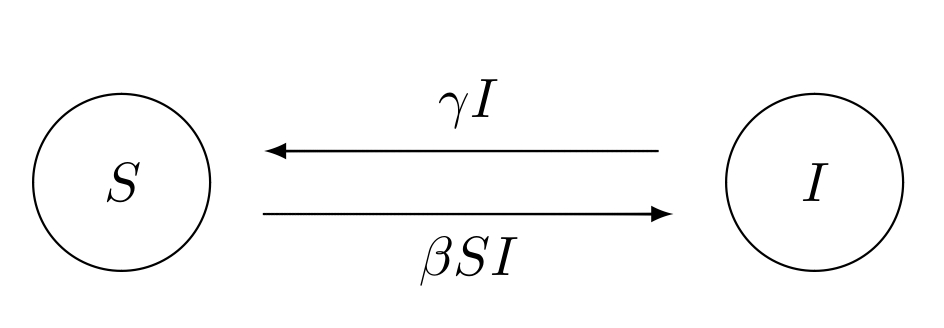
\includegraphics[width=0.4\textwidth]{Figure1.jpg}
\caption{ND-SIS Model}
\label{fig:1}
\end{figure}
\begin{figure}[h!]
\centering
 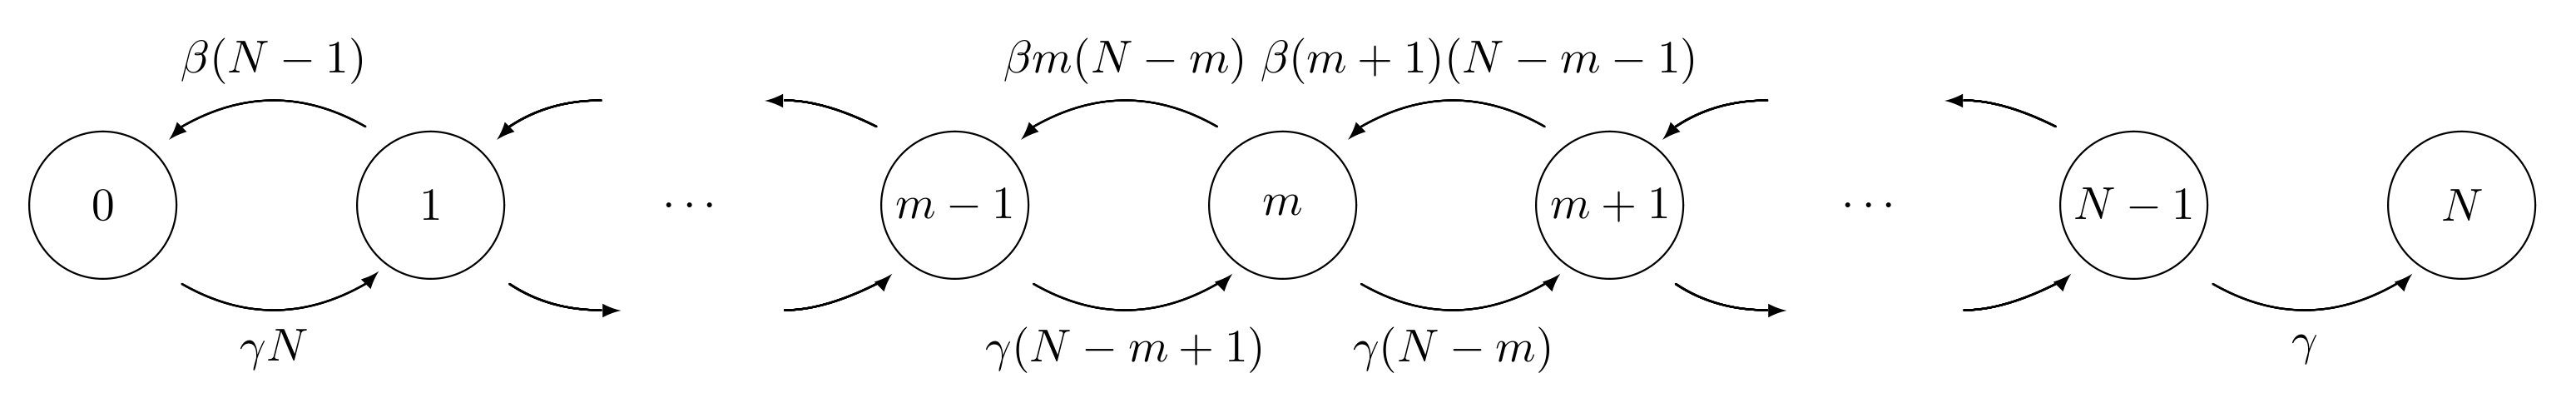
\includegraphics[width=0.8\textwidth]{Figure2.jpg}
\caption{Birth-and-death process ${\cal X}$.}
\label{fig:2}
\end{figure}

\par We consider an initially marked individual $A$ within the population, and our aim is to quantify the probability of individual $A$ suffering
(at least one) re-infection during the process. In order to compute this probability, it is necessary to keep track of the state of individual $A$
throughout time. To this aim, we consider the extended process ${\cal X}^{ext}=\{{\bf X}^{ext}(t)=(S(t),A(t)):\ t\geq0\}$, where $A(t)$ represents the state of individual
$A$ at time $t\geq0$, taking values $S$, $S_I$ and $I$. These values represent that individual $A$, at time $t$, is susceptible and never suffered the
disease before ($S$), is susceptible but suffered the infection before ($S_I$) or is infective ($I$). From now on, we consider here the {\it most
general case} and assume that individual $A$ may have an specific behaviour against the disease (that is, that individual $A$ recovers faster or slower than
the rest of the individuals, or that he/she has a different susceptibility and/or infectivity). Thus, we may define
$\gamma_A$ the recovery rate of individual $A$, while individual $A$ infects the rest of individuals in the population with rate $\beta_{A\rightarrow\cdot}$ and these individuals infect
individual $A$ with rate $\beta_{\cdot\rightarrow A}$. Note that under completely homogeneous conditions (that is, if individual $A$ has the same behaviour against the disease than the rest of
individuals within the population), we have $\gamma_A=\gamma$ and $\beta_{\cdot\rightarrow A}=\beta_{A\rightarrow\cdot}=\beta$.

\par The state space of our extended process ${\cal X}^{ext}$ is given by
\begin{eqnarray*}
 {\cal S}^{ext} &=& \left(\{1,\dots,N-1\}\times\{S,S_I,I\}\right)\cup\{(0,I)\}\cup\left(\{N\}\times\{S,S_I\}\right)\cup\{\Delta\},
\end{eqnarray*}

\par\noindent where $\Delta$ is an {\it artificial} absorbing state representing the re-infection of individual $A$ for the first time, and $(N,S)$
and $(N,S_I)$ are absorbing states representing that the epidemic died out without having re-infection of individual $A$. Possible
transitions between states are given in Table \ref{tab:1}, which together with the space of states ${\cal S}^{ext}$ yield the transitions
diagram given in Figure \ref{fig:3}.
\begin{table}[h]
\centering
\begin{tabular}{|l|l|l|l|}
\hline
Type of event & Original state ($0\leq m\leq N-1$, $n\geq1$) & Destination state & Rate\\
\hline
Recovery of an infective individual & $(m,S)$, $m\geq1$ & $(m+1,S)$ & $\gamma(N-m)$\\
 & $(m,S_I)$, $m\geq1$ & $(m+1,S_I)$ & $\gamma(N-m)$\\
 & $(m,I)$ & $(m+1,S_I)$ & $\gamma_A$\\
 & $(m,I)$, $m\leq N-2$ & $(m+1,I)$ & $\gamma(N-m-1)$\\
\hline
Infection of a susceptible individual & $(m,S)$, $m\geq1$ & $(m-1,I)$ & $\beta_{\cdot\rightarrow A}(N-m)$\\
 & $(m,S)$, $m\geq1$ & $(m-1,S)$ & $\beta(m-1)(N-m)$\\
 & $(m,S_I)$, $m\geq1$ & $\Delta$ & $\beta_{\cdot\rightarrow A}(N-m)$\\
 & $(m,S_I)$, $m\geq1$ & $(m-1,S_I)$ & $\beta(m-1)(N-m)$\\
 & $(m,I)$ & $(m-1,I)$ & $\beta m(N-m-1)+\beta_{A\rightarrow\cdot}m$\\
\hline
\end{tabular}
\caption{Transitions among states in ${\cal S}^{ext}$.}
\label{tab:1}
\end{table}

\begin{figure}[h!]
\centering
 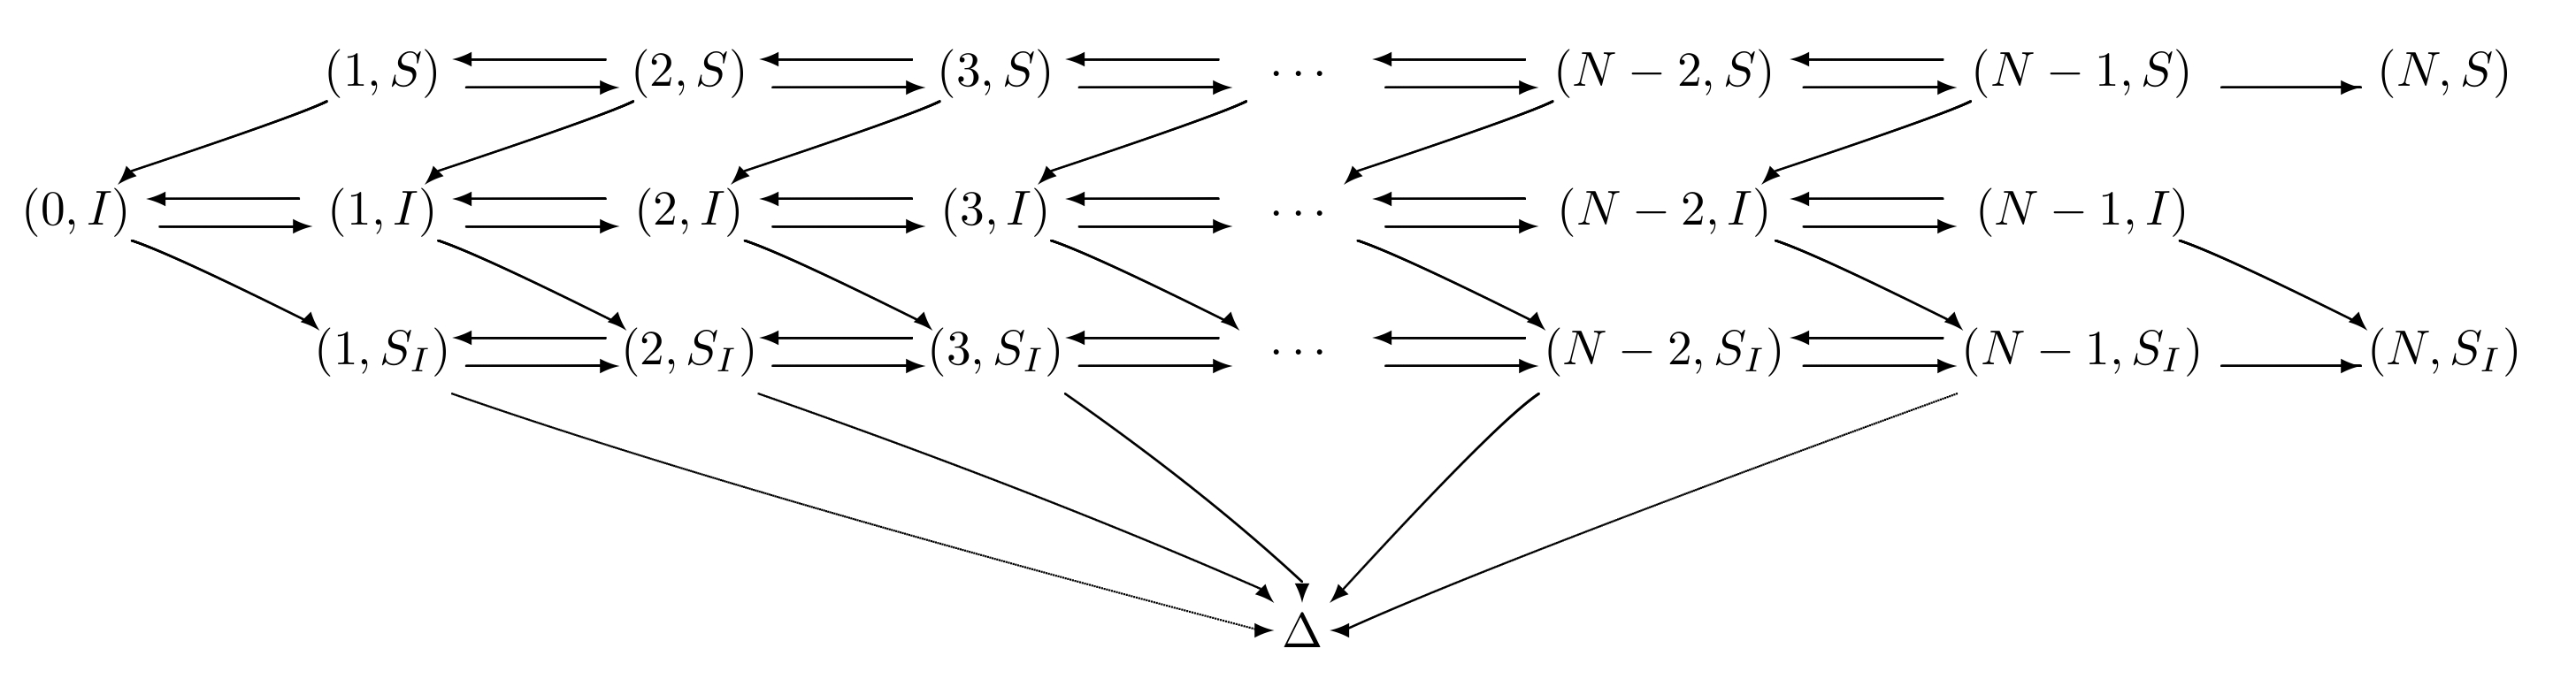
\includegraphics[width=0.8\textwidth]{Figure3.jpg}
\caption{Transitions diagram of ${\cal X}^{ext}$.}
\label{fig:3}
\end{figure}

\par We define
\begin{eqnarray*}
 p_{(m,a)} &=& \hbox{\it ``probability of individual $A$ suffering (at least one) re-infection given the current state of the process $(m,a)\in{\cal S}^{ext}$''},
\end{eqnarray*}
\par\noindent with trivial values $p_{\Delta}=1$, $p_{(N,S)}=p_{(N,S_I)}=0$. These probabilities verify, by a first-step argument, equations
\begin{eqnarray}
 \theta_{(m,S)}p_{(m,S)} &=& \beta(m-1)(N-m)p_{(m-1,S)}+\beta_{\cdot\rightarrow A}(N-m)p_{(m-1,I)}+\gamma(N-m)p_{(m+1,S)},\quad 1\leq m\leq N-1,\label{eqn:1}\\
 \theta_{(m,I)}p_{(m,I)} &=& \left(\beta m(N-m-1)+\beta_{A\rightarrow\cdot}m\right)p_{(m-1,I)}+\gamma (N-m-1)p_{(m+1,I)}+\gamma_Ap_{(m+1,S_I)},\quad 0\leq m\leq N-1,\label{eqn:2}\\
 \theta_{(m,S_I)}p_{(m,S_I)} &=& \beta(m-1)(N-m)p_{(m-1,S_I)}+\beta_{\cdot\rightarrow A}(N-m)p_{\Delta}+\gamma(N-m)p_{(m+1,S_I)},\quad 1\leq m\leq N-1,\label{eqn:3}
\end{eqnarray}
\par\noindent with $\theta_{(m,S)}=\theta_{(m,S_I)}=\beta(m-1)(N-m)+\beta_{\cdot\rightarrow A}(N-m)+\gamma(N-m)$ and $\theta_{(m,I)}=\beta m(N-m-1)+\beta_{A\rightarrow\cdot}m+\gamma(N-m-1)+\gamma_A$. A preliminary analysis of Eqs. \eqref{eqn:1}-\eqref{eqn:3} allows us to find a recursive scheme for
computing these probabilities. In particular, Eq. \eqref{eqn:3} allows us to compute probabilities of the form $p_{(m,S_I)}$ which,
once in hand, allow one the computation of probabilities of the form $p_{(m,I)}$ by Eq. \eqref{eqn:2}. Finally, Eq. \eqref{eqn:1} yields probabilities
of the form $p_{(m,S)}$.

\par When solving Eq. \eqref{eqn:3}, it is possible (by using boundary conditions $p_{\Delta}=1$, $p_{(N,S_I)}=0$) to obtain the iterative
scheme
\begin{eqnarray*}
 p_{(N-1,S_I)} &=& h_{(N-1,S_I)}^{-1}\left(f_{(N-1,S_I)}p_{(N-2,S_I)}+g_{(N-1,S_I)}\right),\ \hbox{\it with } h_{(N-1,S_I)}=1,\ f_{(N-1,S_I)} ~=~ \frac{\beta(N-2)}{\theta_{(N-1,S_I)}},\ g_{(N-1,S_I)}=\frac{\beta_{\cdot\rightarrow A}}{\theta_{(N-1,S_I)}},\\
 p_{(m,S_I)} &=& h_{(m,S_I)}^{-1}\left(f_{(m,S_I)}p_{(m-1,S_I)}+g_{(m,S_I)}\right),\ \hbox{\it with } h_{(m,S_I)}=1-\frac{\gamma(N-m)}{\theta_{(m,S_I)}}h_{(m+1,S_I)}^{-1}f_{(m+1,S_I)},\ f_{(m,S_I)} ~=~ \frac{\beta(m-1)(N-m)}{\theta_{(m,S_I)}},\\
&& g_{(m,S_I)}=\frac{\beta_{\cdot\rightarrow A}(N-m)}{\theta_{{(m,S_I)}}}+\frac{\gamma(N-m)}{\theta_{{(m,S_I)}}}h_{(m+1,S_I)}^{-1}g_{(m+1,S_I)}, \quad \hbox{\it for } m=N-2,\dots,2,\\
 p_{(1,S_I)} &=& h_{(1,S_I)}^{-1}g_{(1,S_I)},\ \hbox{\it with } h_{(1,S_I)}=1-\frac{\gamma(N-1)}{\theta_{(1,S_I)}}h_{(2,S_I)}^{-1}f_{(2,S_I)},\ g_{(1,S_I)}=\frac{\beta_{\cdot\rightarrow A} (N-1)}{\theta_{(1,S_I)}}+\frac{\gamma(N-1)}{\theta_{(1,S_I)}}h_{(2,S_I)}^{-1}g_{(2,S_I)},
\end{eqnarray*}

\par\noindent which yields an algorithmic procedure for computing these probabilities. Once these are in hand, Eq. \eqref{eqn:2} allows us to write
\begin{eqnarray*}
 p_{(N-1,I)} &=& h_{(N-1,I)}^{-1}\left(f_{(N-1,I)}p_{(N-2,I)}+g_{(N-1,I)}\right),\ \hbox{\it with } h_{(N-1,I)}=1,\ f_{(N-1,I)}=\frac{\beta_{A\rightarrow\cdot}(N-1)}{\theta_{(N-1,I)}},\ g_{(N-1,I)}=\frac{\gamma_A}{\theta_{(N-1,I)}}p_{(N,S_I)},\\
 p_{(m,I)} &=& h_{(m,I)}^{-1}\left(f_{(m,I)}p_{(m-1,I)}+g_{(m,I)}\right),\ \hbox{\it with } h_{(m,I)}=1-\frac{\gamma(N-m-1)}{\theta_{(m,I)}}h_{(m+1,I)}^{-1}f_{(m+1,I)},\ f_{(m,I)} ~=~ \frac{\beta m(N-m-1)+\beta_{A\rightarrow\cdot}m}{\theta_{(m,I)}},\\
&& g_{(m,I)}=\frac{\gamma (N-m-1)}{\theta_{(m,I)}}h_{(m+1,I)}^{-1}g_{(m+1,I)}+\frac{\gamma_A}{\theta_{(m,I)}}p_{(m+1,S_I)},\quad \hbox{\it for } m=N-2,\dots,1,\\
 p_{(0,I)} &=& h_{(0,I)}^{-1}g_{(0,I)},\ \hbox{\it with } h_{(0,I)}=1-\frac{\gamma(N-1)}{\theta_{(0,I)}}h_{(1,I)}^{-1}f_{(1,I)},\ g_{(0,I)}=\frac{\gamma(N-1)}{\theta_{(0,I)}}h_{(1,I)}^{-1}g_{(1,I)}+\frac{\gamma_A}{\theta_{(0,I)}}p_{(1,S_I)}.
\end{eqnarray*}

\par\noindent Finally, probabilities of the form $p_{(m,S)}$ are obtained from Eq. \eqref{eqn:1} as
\begin{eqnarray*}
 p_{(N-1,S)} &=& h_{(N-1,S)}^{-1}\left(f_{(N-1,S)}p_{(N-2,S)}+g_{(N-1,S)}\right),\ \hbox{\it with } h_{(N-1,S)}=1,\ f_{(N-1,S)} ~=~ \frac{\beta(N-2)}{\theta_{(N-1,S)}},\ g_{(N-1,S)}=\frac{\beta_{\cdot\rightarrow A}}{\theta_{(N-1,S)}}p_{(N-2,I)},\\
 p_{(m,S)} &=& h_{(m,S)}^{-1}\left(f_{(m,S)}p_{(m-1,S)}+g_{(m,S)}\right),\ \hbox{\it with } h_{(m,S)}=1-\frac{\gamma(N-m)}{\theta_{(m,S)}}h_{(m+1,S)}^{-1}f_{(m+1,S)},\ f_{(m,S)} ~=~ \frac{\beta (m-1)(N-m)}{\theta_{(m,S)}},\\
&& g_{(m,S)}=\frac{\beta_{\cdot\rightarrow A}(N-m)}{\theta_{(m,S)}}p_{(m-1,I)}+\frac{\gamma(N-m)}{\theta_{(m,S)}}h_{(m+1,S)}^{-1}g_{(m+1,S)},\quad \hbox{\it for } m=N-2,\dots,2,\\
 p_{(1,S)} &=& h_{(1,S)}^{-1}g_{(1,S)},\ \hbox{\it with } h_{(1,S)}=1-\frac{\gamma(N-1)}{\theta_{(1,S)}}h_{(2,S)}^{-1}f_{(2,S)},\ g_{(1,S)}=\frac{\beta_{\cdot\rightarrow A} (N-1)}{\theta_{(1,S)}}p_{(0,I)}+\frac{\gamma(N-1)}{\theta_{(1,S)}}h_{(2,S)}^{-1}g_{(2,S)}.
\end{eqnarray*}

\par\noindent From previous recursions, {\bf Algorithm 1} is obtained for computing probabilities in Eqs. \eqref{eqn:1}-\eqref{eqn:3}.\\

\par\noindent{\bf Algorithm 1}\\
\begin{minipage}{9cm}
\begin{description}
  \item $h_{(N-1,S_I)} ~=~ 1$;
  \item $f_{(N-1,S_I)} ~=~ \frac{\beta(N-2)}{\theta_{(N-1,S_I)}}$;
  \item $g_{(N-1,S_I)} ~=~ \frac{\beta_{\cdot\rightarrow A}}{\theta_{(N-1,S_I)}}$;
  \item \it For $m=N-2,\dots,1$:
  \item $~$\hspace{0.5cm} $h_{(m,S_I)} ~=~ 1-\frac{\gamma(N-m)}{\theta_{(m,S_I)}}h_{(m+1,S_I)}^{-1}f_{(m+1,S_I)}$;
  \item $~$\hspace{0.5cm} $f_{(m,S_I)} ~=~ \frac{\beta(m-1)(N-m)}{\theta_{(m,S_I)}}$;
  \item $~$\hspace{0.5cm} $g_{(m,S_I)} ~=~ \frac{\beta_{\cdot\rightarrow A}(N-m)}{\theta_{{(m,S_I)}}}+\frac{\gamma(N-m)}{\theta_{{(m,S_I)}}}h_{(m+1,S_I)}^{-1}g_{(m+1,S_I)}$;
\end{description}
\end{minipage}\begin{minipage}{9cm}
\begin{description}
  \item $p_{(0,I)} ~=~ h_{(0,I)}^{-1}g_{(0,I)}$;
  \item \it For $m=1,\dots,N-1$:
  \item $~$\hspace{0.5cm} $p_{(m,I)} ~=~ h_{(m,I)}^{-1}\left(f_{(m,I)}p_{(m-1,I)}+g_{(m,I)}\right)$;
  \item $h_{(N-1,S)} ~=~ 1$;
  \item $f_{(N-1,S)} ~=~ \frac{\beta(N-2)}{\theta_{(N-1,S)}}$;
  \item $g_{(N-1,S)} ~=~ \frac{\beta_{\cdot\rightarrow A}}{\theta_{(N-1,S)}}p_{(N-2,I)}$;
  \item $~$
\end{description}
\end{minipage}

\begin{minipage}{9cm}
\begin{description}
  \item $p_{(1,S_I)} ~=~ h_{(1,S_I)}^{-1}g_{(1,S_I)}$;
  \item \it For $m=2,\dots,N-1$:
  \item $~$\hspace{0.5cm} $p_{(m,S_I)} ~=~ h_{(m,S_I)}^{-1}\left(f_{(m,S_I)}p_{(m-1,S_I)}+g_{(m,S_I)}\right)$;
  \item $h_{(N-1,I)} ~=~ 1$;
  \item $f_{(N-1,I)} ~=~ \frac{\beta_{A\rightarrow\cdot}(N-1)}{\theta_{(N-1,I)}}$;
  \item $g_{(N-1,I)} ~=~ \frac{\gamma_A}{\theta_{(N-1,I)}}p_{(N,S_I)}$;
  \item \it For $m=N-2,\dots,0$:
  \item $~$\hspace{0.5cm} $h_{(m,I)} ~=~ 1-\frac{\gamma(N-m-1)}{\theta_{(m,I)}}h_{(m+1,I)}^{-1}f_{(m+1,I)}$;
  \item $~$\hspace{0.5cm} $f_{(m,I)} ~=~ \frac{\beta m(N-m-1)+\beta_{A\rightarrow\cdot}m}{\theta_{(m,I)}}$;
  \item $~$\hspace{0.5cm} $g_{(m,I)} ~=~ \frac{\gamma (N-m-1)}{\theta_{(m,I)}}h_{(m+1,I)}^{-1}g_{(m+1,I)}+\frac{\gamma_A}{\theta_{(m,I)}}p_{(m+1,S_I)}$;
\end{description}
\end{minipage}\begin{minipage}{9cm}
\begin{description}
  \item \it For $m=N-2,\dots,1$:
  \item $~$\hspace{0.5cm} $h_{(m,S)} ~=~ 1-\frac{\gamma(N-m)}{\theta_{(m,S)}}h_{(m+1,S)}^{-1}f_{(m+1,S)}$;
  \item $~$\hspace{0.5cm} $f_{(m,S)} ~=~ \frac{\beta (m-1)(N-m)}{\theta_{(m,S)}}$;
  \item $~$\hspace{0.5cm} $g_{(m,S)} ~=~ \frac{\beta_{\cdot\rightarrow A}(N-m)}{\theta_{(m,S)}}p_{(m-1,I)}+\frac{\gamma(N-m)}{\theta_{(m,S)}}h_{(m+1,S)}^{-1}g_{(m+1,S)}$;
  \item $p_{(1,S)} ~=~ h_{(1,S)}^{-1}g_{(1,S)}$;
  \item \it For $m=2,\dots,N-1$:
  \item $~$\hspace{0.5cm} $p_{(m,S)} ~=~ h_{(m,S)}^{-1}\left(f_{(m,S)}p_{(m-1,S)}+g_{(m,S)}\right)$;
  \item $~$
  \item $~$
  \item $~$
  \item $~$
\end{description}
\end{minipage}

\vspace{1cm}

\par\noindent We note here that $h_{(m,S)}=h_{(m,S_I)}$ and $f_{(m,S)}=f_{(m,S_I)}$ for any $m$ in previous algorithms.

\subsection{Temporary and/or partial immunity SIR models}

\par We focus now on epidemic models where some immunity is obtained by individuals suffering the infection. To this aim, we consider modifications
over the standard $S\rightarrow I\rightarrow R$ epidemic model, where temporary and/or partial immunity processes occur:
\begin{itemize}
 \item {\it Temporary immunity:} upon infection, individuals develop an immune response, that is lost after a certain random time (new events $I\rightarrow S$, $R\rightarrow S$).
  \item {\it Partial immunity:} individuals are protected while infected, and regain some susceptibility upon recovery (new event $R\rightarrow I$).
\end{itemize}

That is, the {\it temporary-partial immunity model} given in \cite[Figure 1(e)]{Gomes04}, TPI-SIR Model here, is represented by diagram in Figure
\ref{fig:4}. The {\it temporary immunity SIR model} (TI-SIR Model here) and {\it partial immunity SIR model} (PI-SIR Model here) described in \cite[Figure 1(c)-(d)]{Gomes04} are obtained,
respectively, from the TPI-SIR Model with $\sigma=0$ and $\alpha_I=\alpha_R=0$.
\begin{figure}[h!]
\centering
 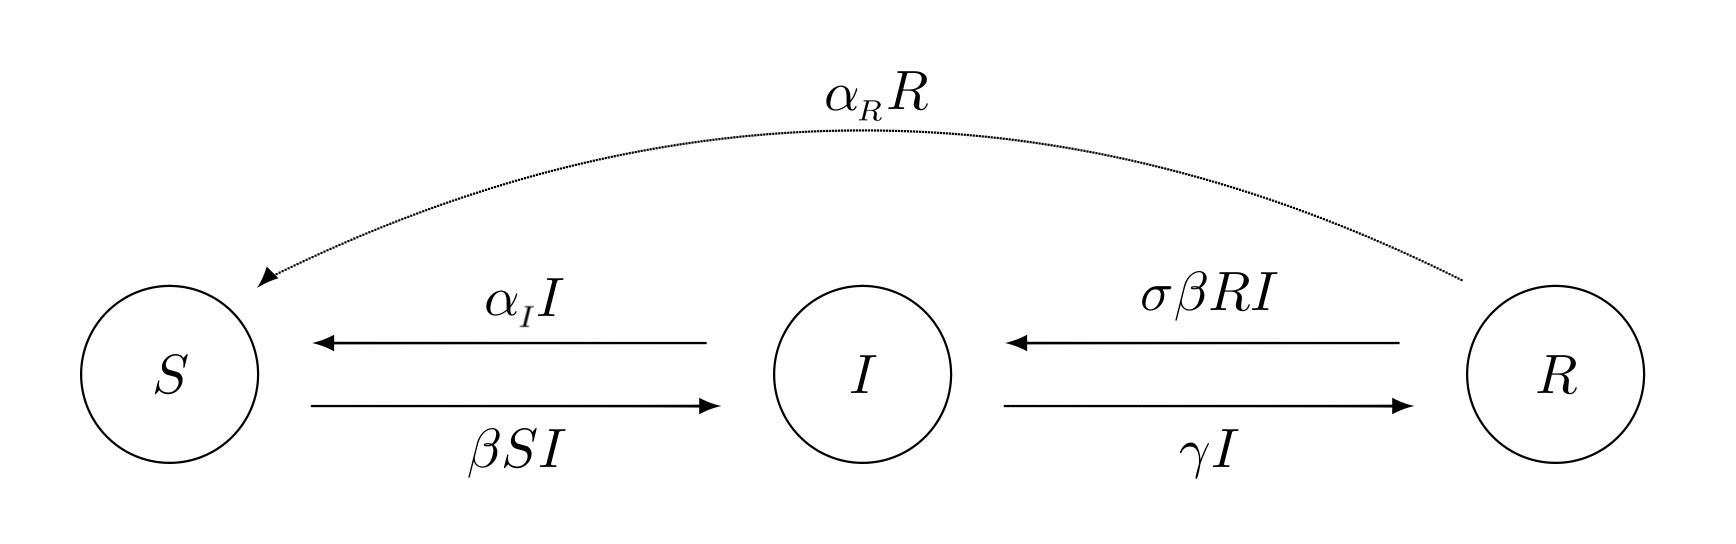
\includegraphics[width=0.5\textwidth]{Figure4.jpg}
\caption{TPI-SIR Model.}
\label{fig:4}
\end{figure}

\par We analyse in this section the probability of re-infection of a marked individual under the TPI-SIR Model, so that the analysis directly
applies to the TI-SIR and PI-SIR Models as particular cases, with some parameters equal to zero. The TPI-SIR Model is represented by the Markovian
process ${\cal \tilde X}=\{{\bf \tilde X}(t)=({\tilde S}(t),{\tilde I}(t)):\ t\geq0\}$, with ${\tilde R}(t)=N-{\tilde S}(t)-{\tilde I}(t)$ the total
number of recovered individuals at time $t$, over the state space ${\cal \tilde S}=\{(m,n)\in\mathbb{N}^2_0: \ m+n\leq N\}$,
and states of the form $(m,0)$ being absorbing states representing the extinction of the epidemic; that is, we consider that the process ends once the
epidemic dies out, even thought there could still occur events involving susceptible and recovered individuals.

\par We propose to track a marked individual $A$ by adding a third variable ${\tilde A}(t)$ to process ${\cal \tilde X}$ as in Subsection 2.1. In particular, we consider
the extended process ${\cal \tilde X}^{ext}=\{{\bf \tilde X}^{ext}=({\tilde S}(t),{\tilde I}(t),{\tilde A}(t)):\ t\geq0\}$ where ${\tilde A}(t)$ takes values among $\{S,S_I,I,R\}$ and represents
the state of individual $A$ at time $t$. The state space of ${\cal \tilde X}^{ext}$ is given by
\begin{eqnarray*}
 {\cal \tilde S}^{ext} &=& \left({\cal \tilde S}^{ext}(S)\times\{S,S_I\}\right)\cup\left({\cal \tilde S}^{ext}(I)\times\{I\}\right)\cup\left({\cal \tilde S}^{ext}(R)\times\{R\}\right)\cup\{\tilde \Delta\},
\end{eqnarray*}
\par\noindent where ${\tilde \Delta}$ is an absorbing state representing re-infection of individual $A$ for the first time,
\begin{eqnarray*}
{\cal \tilde S}^{ext}(S) &=& \{(m,n)\in\mathbb{N}_0^2:\ m>0,\ m+n\leq N\},\\
{\cal \tilde S}^{ext}(I) &=& \{(m,n)\in\mathbb{N}_0^2:\ n>0,\ m+n\leq N\},\\
{\cal \tilde S}^{ext}(R) &=& \{(m,n)\in\mathbb{N}_0^2:\ m+n<N\},
\end{eqnarray*}
\par\noindent and where transitions among states within ${\cal \tilde S}^{ext}$ are given in Table \ref{tab:2}. Heterogeneities related to individual $A$ are given by special rates $\beta_{\cdot\rightarrow A}$, $\beta_{A\rightarrow\cdot}$, $\sigma_A$, $\alpha_R(A)$, $\alpha_I(A)$ and $\gamma_A$. Under homogeneous conditions, we have $\beta_{\cdot\rightarrow A}=\beta_{A\rightarrow\cdot}=\beta$, $\gamma_A=\gamma$, $\sigma_A=\sigma$, $\alpha_R(A)=\alpha_R$ and $\alpha_I(A)=\alpha_I$.

\begin{table}[h]
\centering
\begin{tabular}{|l|l|l|l|}
\hline
Type of event & Original state ($n\geq1$, $m+n\leq N$, & Destination state & Rate\\
 & $0\leq m\leq N-1$) & & \\
\hline
Recovery of an infective individual & $(m,n,S)$, $m\geq1$ & $(m,n-1,S)$ & $\gamma n$\\
 & $(m,n,S_I)$, $m\geq1$ & $(m,n-1,S_I)$ & $\gamma n$\\
 & $(m,n,I)$, $n\geq2$ & $(m,n-1,I)$ & $\gamma(n-1)$\\
 & $(m,n,I)$ & $(m,n-1,R)$ & $\gamma_A$\\
 & $(m,n,R)$, $m+n<N$ & $(m,n-1,R)$ & $\gamma n$\\
\hline
Infection of a susceptible individual & $(m,n,S)$, $m\geq1$ & $(m-1,n+1,I)$ & $\beta_{\cdot\rightarrow A}n$\\
 & $(m,n,S)$, $m\geq2$ & $(m-1,n+1,S)$ & $\beta(m-1)n$\\
 & $(m,n,S_I)$, $m\geq1$ & ${\tilde \Delta}$ & $\beta_{\cdot\rightarrow A}n$\\
 & $(m,n,S_I)$, $m\geq2$ & $(m-1,n+1,S_I)$ & $\beta(m-1)n$\\
 & $(m,n,I)$, $m\geq1$ & $(m-1,n+1,I)$ & $\beta_{A\rightarrow\cdot}m+\beta(n-1)m$\\
 & $(m,n,R)$, $m\geq1,\ m+n<N$ & $(m-1,n+1,R)$ & $\beta mn$\\
\hline
Infection of a recovered individual & $(m,n,S)$, $m\geq1,\ m+n<N$ & $(m,n+1,S)$ & $\sigma\beta n(N-m-n)$\\
 & $(m,n,S_I)$, $m\geq1$, $m+n<N$ & $(m,n+1,S_I)$ & $\sigma\beta n(N-m-n)$\\
 & $(m,n,I)$, $m+n<N$ & $(m,n+1,I)$ & $\sigma\beta(n-1)(N-m-n)+\sigma\beta_{A\rightarrow\cdot}(N-m-n)$\\
 & $(m,n,R)$, $m+n<N-1$ & $(m,n+1,R)$ & $\sigma\beta n(N-m-n-1)$\\
 & $(m,n,R)$, $m+n<N$ & ${\tilde \Delta}$ & $\sigma_A\beta_{\cdot\rightarrow A} n$\\
\hline
Immunity loss of an infective individual & $(m,n,S)$, $m\geq1$ & $(m+1,n-1,S)$ & $\alpha_I n$\\
 & $(m,n,S_I)$, $m\geq1$ & $(m+1,n-1,S_I)$ & $\alpha_I n$\\
 & $(m,n,I)$, $n\geq2$ & $(m+1,n-1,I)$ & $\alpha_I(n-1)$\\
 & $(m,n,I)$ & $(m+1,n-1,S_I)$ & $\alpha_I(A)$\\
 & $(m,n,R)$, $m+n<N$ & $(m+1,n-1,R)$ & $\alpha_I n$\\
\hline
Immunity loss of a recovered individual & $(m,n,S)$, $m\geq1,\ m+n<N$ & $(m+1,n,S)$ & $\alpha_R (N-m-n)$\\
 & $(m,n,S_I)$, $m\geq1,\ m+n<N$ & $(m+1,n,S_I)$ & $\alpha_R (N-m-n)$\\
 & $(m,n,I)$, $m+n<N$ & $(m+1,n,I)$ & $\alpha_R (N-m-n)$\\
 & $(m,n,R)$, $m+n<N-1$ & $(m+1,n,R)$ & $\alpha_R (N-m-n-1)$\\
 & $(m,n,R)$, $m+n<N$ & $(m+1,n,S_I)$ & $\alpha_R(A)$\\
\hline
\end{tabular}
\caption{Transitions among states in ${\cal \tilde S}^{ext}$.}
\label{tab:2}
\end{table}

\par We define $p_{(m,n,a)}$ as the probability of individual $A$ suffering (at least one) re-infection given the current state of the process $(m,n,a)\in{\cal \tilde S}^{ext}$.
These probabilities verify, for $m\geq0$, $n\geq1$ and $m+n\leq N$, equations
\begin{eqnarray}
 \theta_{(m,n,S)}p_{(m,n,S)} &=& \beta(m-1)np_{(m-1,n+1,S)}+\beta_{\cdot\rightarrow A}np_{(m-1,n+1,I)}+\gamma np_{(m,n-1,S)}+\alpha_I np_{(m+1,n-1,S)}+\alpha_R(N-m-n)\nonumber\\
&& \times p_{(m+1,n,S)}+\sigma\beta n(N-m-n)p_{(m,n+1,S)},\quad m\geq1,\label{eqn:4}\\
 \theta_{(m,n,I)}p_{(m,n,I)} &=& \left(\beta m(n-1)+\beta_{A\rightarrow\cdot}m\right)p_{(m-1,n+1,I)}+\gamma (n-1)p_{(m,n-1,I)}+\gamma_Ap_{(m,n-1,R)}+\alpha_I(n-1)p_{(m+1,n-1,I)}\nonumber\\
&& +\alpha_I(A)p_{(m+1,n-1,S_I)}+\left(\sigma\beta(n-1)(N-m-n)+\sigma\beta_{A\rightarrow\cdot}(N-m-n)\right)p_{(m,n+1,I)}+\alpha_R(N-m-n)p_{(m+1,n,I)},\quad \label{eqn:5}\\
 \theta_{(m,n,R)}p_{(m,n,R)} &=& \beta mnp_{(m-1,n+1,R)}+\gamma np_{(m,n-1,R)}+\alpha_I np_{(m+1,n-1,R)}+\alpha_R(N-m-n-1)p_{(m+1,n,R)}+\alpha_R(A)\nonumber\\
&&\times p_{(m+1,n,S_I)}+\sigma\beta n(N-m-n-1)p_{(m,n+1,R)}+\sigma_A\beta_{\cdot\rightarrow A} np_{{\tilde \Delta}},\quad m+n< N,\label{eqn:6}\\
 \theta_{(m,n,S_I)}p_{(m,n,S_I)} &=& \beta(m-1)np_{(m-1,n+1,S_I)}+\beta_{\cdot\rightarrow A}np_{{\tilde \Delta}}+\gamma np_{(m,n-1,S_I)}+\alpha_I np_{(m+1,n-1,S_I)}+\alpha_R(N-m-n)\nonumber\\
&& \times p_{(m+1,n,S_I)}+\sigma\beta n(N-m-n)p_{(m,n+1,S_I)},\quad m\geq1.\label{eqn:7}
\end{eqnarray}
\par\noindent with $\theta_{(m,n,S)}=\theta_{(m,n,S_I)}=\beta(m-1)n+\beta_{\cdot\rightarrow A}n+\gamma n+\alpha_I n+\alpha_R(N-m-n)+\sigma\beta n(N-m-n)$, $\theta_{(m,n,I)}=\beta m(n-1)+\beta_{A\rightarrow\cdot}m+\gamma (n-1)+\gamma_A+\alpha_I(n-1)+\alpha_I(A)+\sigma\beta(n-1)(N-m-n)+\sigma\beta_{A\rightarrow\cdot}(N-m-n)+\alpha_R(N-m-n)$, $\theta_{(m,n,R)}=\beta mn+\gamma n+\alpha_I n+\alpha_R(N-m-n-1)+\alpha_R(A)+\sigma\beta n(N-m-n-1)+\sigma_A\beta_{\cdot\rightarrow A}n$, and boundary conditions $p_{{\tilde \Delta}}=1$, $p_{(m,0,S)}=p_{(m,0,S_I)}=p_{(m,0,R)}=0$, for any value of $m$.

\par Eqs. \eqref{eqn:4}-\eqref{eqn:7} can be solved algorithmically in a backwards fashion. In particular, Eq. \eqref{eqn:7} can be solved first by
considering
\begin{eqnarray*}
 {\cal \tilde S}^{ext}(S) &=& \{(m,n)\in\mathbb{N}_0^2:\ m>0,\ m+n\leq N\} \ = \ \left(\{(m,0):\ 1\leq m\leq N\}\right)\cup{\cal C}^{ext}(S),\\
 {\cal C}^{ext}(S) &=& \{(m,n)\in\mathbb{N}^2:\ m+n\leq N\} \ = \ \bigcup\limits_{k=2}^{N} L(S;k),\\
 L(S;k) &=& \{(m,n)\in\mathbb{N}^2:\ m+n=k\},\quad 2\leq k\leq N.
\end{eqnarray*}

\par\noindent With this states organisation, Eq. \eqref{eqn:7} can be written in matrix form as
\begin{eqnarray}\label{eqn:8}
 {\bf p}(S_I) &=& {\bf A}(S_I){\bf p}(S_I)+{\bf b}(S_I),
\end{eqnarray}
\par\noindent with
\begin{eqnarray*}
 {\bf p}(S_I) &=& \left(\begin{array}{c}
                         {\bf p}_2(S_I)\\
{\bf p}_3(S_I)\\
\vdots\\
{\bf p}_N(S_I)
\end{array}\right),\quad {\bf p}_k(S_I) \ = \ \left(\begin{array}{c}
p_{(k-1,1,S_I)}\\
p_{(k-2,2,S_I)}\\
\vdots\\
p_{(1,k-1,S_I)}
\end{array}\right),\quad
{\bf b}(S_I) \ = \ \left(\begin{array}{c}
                          {\bf b}_2(S_I)\\
{\bf b}_3(S_I)\\
\vdots\\
{\bf b}_N(S_I)
                         \end{array}\right),\quad
{\bf b}_k(S_I) \ = \ \left(\begin{array}{c}
               \frac{\beta_{\cdot\rightarrow A}}{\theta_{(k-1,1,S_I)}}\\
\frac{\beta_{\cdot\rightarrow A}2}{\theta_{(k-2,2,S_I)}}\\
\vdots\\
\frac{\beta_{\cdot\rightarrow A}(k-1)}{\theta_{(1,k-1,S_I)}}\\
                         \end{array}\right),
\end{eqnarray*}

\par\noindent and with matrix ${\bf A}(S_I)$ given by
\begin{equation*}
  \left(\begin{array}{cccccc}
{\bf A}_{2,2}(S_I) & {\bf A}_{2,3}(S_I) & {\bf 0}_{J(S;2)\times J(S;4)} & \dots & {\bf 0}_{J(S;2)\times J(S;N-1)} & {\bf 0}_{J(S;2)\times J(S;N)}\\
{\bf A}_{3,2}(S_I) & {\bf A}_{3,3}(S_I) & {\bf A}_{3,4}(S_I) & \dots & {\bf 0}_{J(S;3)\times J(S;N-1)} & {\bf 0}_{J(S;3)\times J(S;N)}\\
{\bf 0}_{J(S;4)\times J(S;2)} & {\bf A}_{4,3}(S_I) & {\bf A}_{4,4}(S_I) & \dots & {\bf 0}_{J(S;4)\times J(S;N-1)} & {\bf 0}_{J(S;4)\times J(S;N)}\\
\vdots & \vdots & \vdots & \ddots & \vdots & \vdots\\
{\bf 0}_{J(S;N-1)\times J(S;2)} & {\bf 0}_{J(S;N-1)\times J(S;3)} & {\bf 0}_{J(S;N-1)\times J(S;4)} & \dots & {\bf A}_{N-1,N-1}(S_I) & {\bf A}_{N-1,N}(S_I) \\
{\bf 0}_{J(S;N)\times J(S;2)} & {\bf 0}_{J(S;N)\times J(S;3)} & {\bf 0}_{J(S;N)\times J(S;4)} & \dots & {\bf A}_{N,N-1}(S_I) & {\bf A}_{N,N}(S_I)
                        \end{array}\right),
\end{equation*}
\par\noindent and with sub-matrices
\begin{eqnarray*}
 {\bf A}_{k,k}(S_I) &=& \left(\begin{array}{cccccc}
0 & \frac{\beta(k-2)}{\theta_{(k-1,1,S_I)}} & 0 & \dots & 0 & 0\\
\frac{\alpha_I2}{\theta_{(k-2,2,S_I)}} & 0 & \frac{\beta2(k-3)}{\theta_{(k-2,2,S_I)}} & \dots & 0 & 0\\
0 & \frac{\alpha_I3}{\theta_{(k-3,3,S_I)}} & 0 & \dots & 0 & 0\\
\vdots & \vdots & \vdots & \ddots & \vdots & \vdots\\
0 & 0 & 0 & \dots & 0 & \frac{\beta(k-2)}{\theta_{(2,k-2,S_I)}}\\
0 & 0 & 0 & \dots & \frac{\alpha_I(k-1)}{\theta_{(1,k-1,S_I)}} & 0
                        \end{array}\right),\quad 2\leq k\leq N,
\end{eqnarray*}
\begin{eqnarray*}
 {\bf A}_{k,k-1}(S_I) &=& \left(\begin{array}{cccccc}
0 & 0 & 0 & \dots & 0 & 0\\
\frac{\gamma2}{\theta_{(k-2,2,S_I)}} & 0 & 0 & \dots & 0 & 0\\
0 & \frac{\gamma3}{\theta_{(k-3,3,S_I)}} & 0 & \dots & 0 & 0\\
\vdots & \vdots & \vdots & \ddots & \vdots & \vdots\\
0 & 0 & 0 & \dots & \frac{\gamma(k-2)}{\theta_{(2,k-2,S_I)}} & 0\\
0 & 0 & 0 & \dots & 0 & \frac{\gamma(k-1)}{\theta_{(1,k-1,S_I)}}
                        \end{array}\right),\quad 3\leq k\leq N,\\
 {\bf A}_{k,k+1}(S_I) &=& \left(\begin{array}{cccccc}
\frac{\alpha_R(N-k)}{\theta_{(k-1,1,S_I)}} & \frac{\sigma\beta(N-k)}{\theta_{(k-1,1,S_I)}} & 0 & \dots & 0 & 0\\
0 & \frac{\alpha_R(N-k)}{\theta_{(k-2,2,S_I)}} & \frac{\sigma\beta(N-k)2}{\theta_{(k-2,2,S_I)}} & \dots & 0 & 0\\
0 & 0 & \frac{\alpha_R(N-k)}{\theta_{(k-3,3,S_I)}} & \dots & 0 & 0\\
\vdots & \vdots & \vdots & \ddots & \vdots & \vdots\\
0 & 0 & 0 & \dots & \frac{\sigma\beta(N-k)(k-2)}{\theta_{(2,k-2,S_I)}} & 0\\
0 & 0 & 0 & \dots & \frac{\alpha_R(N-k)}{\theta_{(1,k-1,S_I)}} & \frac{\sigma\beta(N-k)(k-1)}{\theta_{(1,k-1,S_I)}}
                        \end{array}\right),\quad 2\leq k\leq N-1,
\end{eqnarray*}

\par\noindent where $J(S;k)=\# L(S;k)=k-1$, and $\#B$ represents the cardinality of set $B$. According to the structure of matrix ${\bf A}(S_I)$,
system in Eq. \eqref{eqn:8} can be algorithmically solved so that {\bf Algorithm 2} is obtained.

\vspace{0.5cm}
\par \noindent{\bf Algorithm 2}
\begin{description}
  \item ${\bf H}_2(S_I) ~=~ {\bf I}_{J(S;2)}-{\bf A}_{2,2}(S_I)$;
  \item ${\bf P}_2(S_I) ~=~ {\bf b}_2(S_I)$;
  \item \it For $k=3,\dots,N$:
  \item $~$\hspace{0.5cm} ${\bf H}_k(S_I) ~=~ {\bf I}_{J(S;k)}-{\bf A}_{k,k}(S_I)-{\bf A}_{k,k-1}(S_I){\bf H}_{k-1}^{-1}(S_I){\bf A}_{k-1,k}(S_I)$;
  \item $~$\hspace{0.5cm} ${\bf P}_k(S_I) ~=~ {\bf A}_{k,k-1}(S_I){\bf H}_{k-1}^{-1}(S_I){\bf P}_{k-1}(S_I)+{\bf b}_k(S_I)$;
  \item ${\bf p}_N(S_I) ~=~ {\bf H}_N^{-1}(S_I){\bf P}_N(S_I)$;
  \item \it For $k=N-1,\dots,2$:
  \item $~$\hspace{0.5cm} ${\bf p}_k(S_I) ~=~ {\bf H}_k^{-1}(S_I)\left({\bf A}_{k,k+1}(S_I){\bf p}_{k+1}(S_I)+{\bf P}_k(S_I)\right)$;
\end{description}
\vspace{0.5cm}


\par Once probabilities of the form $p_{(m,n,S_I)}$ are in hand, one proceeds to obtain probabilities $p_{(m,n,R)}$ from Eq. \eqref{eqn:6}, which can be
re-written in matrix form by organising
\begin{eqnarray*}
 {\cal \tilde S}^{ext}(R) &=& \{(m,n)\in\mathbb{N}_0^2:\ m+n< N\} \ = \ \left(\{(m,0):\ 0\leq m\leq N-1\}\right)\cup{\cal C}^{ext}(R),\\
 {\cal C}^{ext}(R) &=& \{(m,n)\in\mathbb{N}_0^2:\ n\geq1,\ m+n< N\} \ = \ \bigcup\limits_{k=1}^{N-1} L(R;k),\\
 L(R;k) &=& \{(m,n)\in\mathbb{N}_0^2:\ n\geq1,\ m+n=k\},\quad 1\leq k\leq N-1.
\end{eqnarray*}

\par\noindent We obtain
\begin{eqnarray}\label{eqn:9}
 {\bf p}(R) &=& {\bf A}(R){\bf p}(R)+{\bf b}(R),
\end{eqnarray}
\par\noindent with
\begin{eqnarray*}
 {\bf p}(R) &=& \left(\begin{array}{c}
                         {\bf p}_1(R)\\
{\bf p}_2(R)\\
\vdots\\
{\bf p}_{N-1}(R)
\end{array}\right),\quad {\bf p}_k(R) \ = \ \left(\begin{array}{c}
p_{(k-1,1,R)}\\
p_{(k-2,2,R)}\\
\vdots\\
p_{(1,k-1,R)}\\
p_{(0,k,R)}
\end{array}\right),
\end{eqnarray*}
\par\noindent column vector
\begin{eqnarray*}
{\bf b}(R) &=& \left(\begin{array}{c}
                          {\bf b}_1(R)\\
{\bf b}_2(R)\\
\vdots\\
{\bf b}_{N-1}(R)
                         \end{array}\right),\quad
{\bf b}_k(R) \ = \ \left(\begin{array}{c}
               \frac{\alpha_R(A)p_{(k,1,S_I)}+\sigma_A\beta_{\cdot\rightarrow A}}{\theta_{(k-1,1,R)}}\\
\frac{\alpha_R(A)p_{(k-1,2,S_I)}+\sigma_A\beta_{\cdot\rightarrow A}2}{\theta_{(k-2,2,R)}}\\
\vdots\\
\frac{\alpha_R(A)p_{(1,k,S_I)}+\sigma_A\beta_{\cdot\rightarrow A}k}{\theta_{(0,k,R)}}
                         \end{array}\right),
\end{eqnarray*}

\par\noindent and with matrix ${\bf A}(R)$ given by
\begin{equation*}
  \left(\begin{array}{cccccc}
{\bf A}_{1,1}(R) & {\bf A}_{1,2}(R) & {\bf 0}_{J(R;1)\times J(R;3)} & \dots & {\bf 0}_{J(R;1)\times J(R;N-2)} & {\bf 0}_{J(R;1)\times J(R;N-1)}\\
{\bf A}_{2,1}(R) & {\bf A}_{2,2}(R) & {\bf A}_{2,3}(R) & \dots & {\bf 0}_{J(R;2)\times J(R;N-2)} & {\bf 0}_{J(R;2)\times J(R;N-1)}\\
{\bf 0}_{J(R;3)\times J(R;1)} & {\bf A}_{3,2}(R) & {\bf A}_{3,3}(R) & \dots & {\bf 0}_{J(R;3)\times J(R;N-2)} & {\bf 0}_{J(R;3)\times J(R;N-1)}\\
\vdots & \vdots & \vdots & \ddots & \vdots & \vdots\\
{\bf 0}_{J(R;N-2)\times J(R;1)} & {\bf 0}_{J(R;N-2)\times J(R;2)} & {\bf 0}_{J(R;N-2)\times J(R;3)} & \dots & {\bf A}_{N-2,N-2}(R) & {\bf A}_{N-2,N-1}(R) \\
{\bf 0}_{J(R;N-1)\times J(R;1)} & {\bf 0}_{J(R;N-1)\times J(R;2)} & {\bf 0}_{J(R;N-1)\times J(R;3)} & \dots & {\bf A}_{N-1,N-2}(R) & {\bf A}_{N-1,N-1}(R)
                        \end{array}\right),
\end{equation*}
\par\noindent and with sub-matrices
\begin{eqnarray*}
 {\bf A}_{k,k}(R) &=& \left(\begin{array}{cccccc}
0 & \frac{\beta(k-1)}{\theta_{(k-1,1,R)}} & 0 & \dots & 0 & 0\\
\frac{\alpha_I2}{\theta_{(k-2,2,R)}} & 0 & \frac{\beta2(k-2)}{\theta_{(k-2,2,R)}} & \dots & 0 & 0\\
0 & \frac{\alpha_I3}{\theta_{(k-3,3,R)}} & 0 & \dots & 0 & 0\\
\vdots & \vdots & \vdots & \ddots & \vdots & \vdots\\
0 & 0 & 0 & \dots & 0 & \frac{\beta(k-1)}{\theta_{(1,k-1,R)}}\\
0 & 0 & 0 & \dots & \frac{\alpha_Ik}{\theta_{(0,k,R)}} & 0
                        \end{array}\right),\quad 1\leq k\leq N-1,\\
 {\bf A}_{k,k-1}(R) &=& \left(\begin{array}{cccccc}
0 & 0 & 0 & \dots & 0 & 0\\
\frac{\gamma2}{\theta_{(k-2,2,R)}} & 0 & 0 & \dots & 0 & 0\\
0 & \frac{\gamma3}{\theta_{(k-3,3,R)}} & 0 & \dots & 0 & 0\\
\vdots & \vdots & \vdots & \ddots & \vdots & \vdots\\
0 & 0 & 0 & \dots & \frac{\gamma(k-1)}{\theta_{(1,k-1,R)}} & 0\\
0 & 0 & 0 & \dots & 0 & \frac{\gamma k}{\theta_{(0,k,R)}}
                        \end{array}\right),\quad 2\leq k\leq N-1,
\end{eqnarray*}
\begin{eqnarray*}
 {\bf A}_{k,k+1}(R) &=& \left(\begin{array}{cccccc}
\frac{\alpha_R(N-k-1)}{\theta_{(k-1,1,R)}} & \frac{\sigma\beta(N-k-1)}{\theta_{(k-1,1,R)}} & 0 & \dots & 0 & 0\\
0 & \frac{\alpha_R(N-k-1)}{\theta_{(k-2,2,R)}} & \frac{\sigma\beta(N-k-1)2}{\theta_{(k-2,2,R)}} & \dots & 0 & 0\\
0 & 0 & \frac{\alpha_R(N-k-1)}{\theta_{(k-3,3,R)}} & \dots & 0 & 0\\
\vdots & \vdots & \vdots & \ddots & \vdots & \vdots\\
0 & 0 & 0 & \dots & \frac{\sigma\beta(N-k-1)(k-1)}{\theta_{(1,k-1,R)}} & 0\\
0 & 0 & 0 & \dots & \frac{\alpha_R(N-k-1)}{\theta_{(0,k,R)}} & \frac{\sigma\beta(N-k-1)k}{\theta_{(0,k,R)}}
                        \end{array}\right),\quad 1\leq k\leq N-2,
\end{eqnarray*}
\par\noindent with $J(R;k)=\#L(R;k)=k$.

\par From Eq. \eqref{eqn:9} and the structure of matrix ${\bf A}(R)$, we obtain {\bf Algorithm 2 (continuation I)}.

\vspace{0.5cm}
\par \noindent{\bf Algorithm 2 (continuation I)}
\begin{description}
  \item ${\bf H}_1(R) ~=~ {\bf I}_{J(R;1)}-{\bf A}_{1,1}(R)$;
  \item ${\bf P}_1(R) ~=~ {\bf b}_1(R)$;
  \item \it For $k=2,\dots,N-1$:
  \item $~$\hspace{0.5cm} ${\bf H}_k(R) ~=~ {\bf I}_{J(R;k)}-{\bf A}_{k,k}(R)-{\bf A}_{k,k-1}(R){\bf H}_{k-1}^{-1}(R){\bf A}_{k-1,k}(R)$;
  \item $~$\hspace{0.5cm} ${\bf P}_k(R) ~=~ {\bf A}_{k,k-1}(R){\bf H}_{k-1}^{-1}(R){\bf P}_{k-1}(R)+{\bf b}_k(R)$;
  \item ${\bf p}_{N-1}(R) ~=~ {\bf H}_{N-1}^{-1}(R){\bf P}_{N-1}(R)$;
  \item \it For $k=N-2,\dots,1$:
  \item $~$\hspace{0.5cm} ${\bf p}_k(R) ~=~ {\bf H}_k^{-1}(R)\left({\bf A}_{k,k+1}(R){\bf p}_{k+1}(R)+{\bf P}_k(R)\right)$;
\end{description}
\vspace{0.5cm}


\par In a similar way, probabilities of the form $p_{(m,n,I)}$ can be obtained from Eq. \eqref{eqn:5} once probabilities $p_{(m,n,R)}$ are in hand.
In particular, by organising
\begin{eqnarray*}
 {\cal \tilde S}^{ext}(I) &=& \{(m,n)\in\mathbb{N}_0^2:\ n\geq1,\ m+n\leq N\} \ = \ {\cal C}^{ext}(I),\\
 {\cal C}^{ext}(I) &=& \bigcup\limits_{k=1}^{N} L(I;k),\\
 L(I;k) &=& \{(m,n)\in\mathbb{N}_0^2:\ n\geq1,\ m+n=k\},\quad 1\leq k\leq N.
\end{eqnarray*}

\par\noindent We obtain
\begin{eqnarray}\label{eqn:10}
 {\bf p}(I) &=& {\bf A}(I){\bf p}(I)+{\bf b}(I),
\end{eqnarray}
\par\noindent with
\begin{eqnarray*}
 {\bf p}(I) &=& \left(\begin{array}{c}
                         {\bf p}_1(I)\\
{\bf p}_2(I)\\
\vdots\\
{\bf p}_{N}(I)
\end{array}\right),\quad {\bf p}_k(I) \ = \ \left(\begin{array}{c}
p_{(k-1,1,I)}\\
p_{(k-2,2,I)}\\
\vdots\\
p_{(1,k-1,I)}\\
p_{(0,k,I)}
\end{array}\right),
\end{eqnarray*}
\par\noindent column vector
\begin{eqnarray*}
{\bf b}(I) &=& \left(\begin{array}{c}
                          {\bf b}_1(I)\\
{\bf b}_2(I)\\
\vdots\\
{\bf b}_{N}(I)
                         \end{array}\right),\quad
{\bf b}_k(I) \ = \ \left(\begin{array}{c}
               0\\
\frac{\gamma_A p_{(k-2,1,R)}+\alpha_I(A) p_{(k-1,1,S_I)}}{\theta_{(k-2,2,I)}}\\
\vdots\\
\frac{\gamma_Ap_{(0,k-1,R)}+\alpha_I(A)p_{(1,k-1,S_I)}}{\theta_{(0,k,I)}}
                         \end{array}\right),
\end{eqnarray*}

\par\noindent and with matrix ${\bf A}(I)$ given by
\begin{equation*}
  \left(\begin{array}{cccccc}
{\bf A}_{1,1}(I) & {\bf A}_{1,2}(I) & {\bf 0}_{J(I;1)\times J(I;3)} & \dots & {\bf 0}_{J(I;1)\times J(I;N-1)} & {\bf 0}_{J(I;1)\times J(I;N)}\\
{\bf A}_{2,1}(I) & {\bf A}_{2,2}(I) & {\bf A}_{2,3}(I) & \dots & {\bf 0}_{J(I;2)\times J(I;N-1)} & {\bf 0}_{J(I;2)\times J(I;N)}\\
{\bf 0}_{J(I;3)\times J(I;1)} & {\bf A}_{3,2}(I) & {\bf A}_{3,3}(I) & \dots & {\bf 0}_{J(I;3)\times J(I;N-1)} & {\bf 0}_{J(I;3)\times J(I;N)}\\
\vdots & \vdots & \vdots & \ddots & \vdots & \vdots\\
{\bf 0}_{J(I;N-1)\times J(I;1)} & {\bf 0}_{J(I;N-1)\times J(I;2)} & {\bf 0}_{J(I;N-1)\times J(I;3)} & \dots & {\bf A}_{N-1,N-1}(I) & {\bf A}_{N-1,N}(I) \\
{\bf 0}_{J(I;N)\times J(I;1)} & {\bf 0}_{J(I;N)\times J(I;2)} & {\bf 0}_{J(I;N)\times J(I;3)} & \dots & {\bf A}_{N,N-1}(I) & {\bf A}_{N,N}(I)
                        \end{array}\right),
\end{equation*}
\par\noindent and with sub-matrices
\begin{eqnarray*}
 {\bf A}_{k,k}(I) &=& \left(\begin{array}{cccccc}
0 & \frac{\beta(k-1)}{\theta_{(k-1,1,I)}} & 0 & \dots & 0 & 0\\
\frac{\alpha_I}{\theta_{(k-2,2,I)}} & 0 & \frac{\beta2(k-2)}{\theta_{(k-2,2,I)}} & \dots & 0 & 0\\
0 & \frac{\alpha_I2}{\theta_{(k-3,3,I)}} & 0 & \dots & 0 & 0\\
\vdots & \vdots & \vdots & \ddots & \vdots & \vdots\\
0 & 0 & 0 & \dots & 0 & \frac{\beta(k-1)}{\theta_{(1,k-1,I)}}\\
0 & 0 & 0 & \dots & \frac{\alpha_I (k-1)}{\theta_{(0,k,I)}} & 0
                        \end{array}\right),\quad 1\leq k\leq N,\\
 {\bf A}_{k,k-1}(I) &=& \left(\begin{array}{cccccc}
0 & 0 & 0 & \dots & 0 & 0\\
\frac{\gamma}{\theta_{(k-2,2,I)}} & 0 & 0 & \dots & 0 & 0\\
0 & \frac{\gamma2}{\theta_{(k-3,3,I)}} & 0 & \dots & 0 & 0\\
\vdots & \vdots & \vdots & \ddots & \vdots & \vdots\\
0 & 0 & 0 & \dots & \frac{\gamma(k-2)}{\theta_{(1,k-1,I)}} & 0\\
0 & 0 & 0 & \dots & 0 & \frac{\gamma (k-1)}{\theta_{(0,k,I)}}
                        \end{array}\right),\quad 2\leq k\leq N,\\
 {\bf A}_{k,k+1}(I) &=& \left(\begin{array}{cccccc}
\frac{\alpha_R(N-k)}{\theta_{(k-1,1,I)}} & \frac{\sigma(N-k)(\beta(n-1)+\beta_{A\rightarrow\cdot})}{\theta_{(k-1,1,I)}} & 0 & \dots & 0 & 0\\
0 & \frac{\alpha_R(N-k)}{\theta_{(k-2,2,I)}} & \frac{\sigma(N-k)(\beta(n-1)+\beta_{A\rightarrow\cdot})}{\theta_{(k-2,2,I)}} & \dots & 0 & 0\\
0 & 0 & \frac{\alpha_R(N-k)}{\theta_{(k-3,3,I)}} & \dots & 0 & 0\\
\vdots & \vdots & \vdots & \ddots & \vdots & \vdots\\
0 & 0 & 0 & \dots & \frac{\sigma(N-k)(\beta(n-1)+\beta_{A\rightarrow\cdot})}{\theta_{(1,k-1,I)}} & 0\\
0 & 0 & 0 & \dots & \frac{\alpha_R(N-k)}{\theta_{(0,k,I)}} & \frac{\sigma(N-k)(\beta(n-1)+\beta_{A\rightarrow\cdot})}{\theta_{(0,k,I)}}
                        \end{array}\right),\\
                        && \quad\quad\quad\quad\quad\quad\quad\quad\quad\quad\quad\quad\quad\quad\quad\quad\quad\quad\quad\quad\quad\quad\quad\quad\quad\quad\quad\quad\quad\quad\quad\quad\quad\quad\quad\quad\quad\quad\quad\quad\quad\quad\quad 1\leq k\leq N-1,
\end{eqnarray*}
\par\noindent with $J(I;k)=\#L(I;k)=k$.\\

\par From Eq. \eqref{eqn:10}, we obtain {\bf Algorithm 2 (continuation II)}.\\

\vspace{0.5cm}
\par \noindent{\bf Algorithm 2 (continuation II)}
\begin{description}
  \item ${\bf H}_1(I) ~=~ {\bf I}_{J(I;1)}-{\bf A}_{1,1}(I)$;
  \item ${\bf P}_1(I) ~=~ {\bf b}_1(I)$;
  \item \it For $k=2,\dots,N$:
  \item $~$\hspace{0.5cm} ${\bf H}_k(I) ~=~ {\bf I}_{J(I;k)}-{\bf A}_{k,k}(I)-{\bf A}_{k,k-1}(I){\bf H}_{k-1}^{-1}(I){\bf A}_{k-1,k}(I)$;
  \item $~$\hspace{0.5cm} ${\bf P}_k(I) ~=~ {\bf A}_{k,k-1}(I){\bf H}_{k-1}^{-1}(I){\bf P}_{k-1}(I)+{\bf b}_k(I)$;
  \item ${\bf p}_{N}(I) ~=~ {\bf H}_{N}^{-1}(I){\bf P}_{N}(I)$;
  \item \it For $k=N-1,\dots,1$:
  \item $~$\hspace{0.5cm} ${\bf p}_k(I) ~=~ {\bf H}_k^{-1}(I)\left({\bf A}_{k,k+1}(I){\bf p}_{k+1}(I)+{\bf P}_k(I)\right)$;
\end{description}
\vspace{0.5cm}

\par Finally, probabilities $p_{(m,n,S)}$ can be computed from Eq. \eqref{eqn:4} by following exactly the same arguments than when solving Eq. \eqref{eqn:7}. In
particular, we note that Eqs. \eqref{eqn:4} and \eqref{eqn:7} only differ in terms $\frac{\beta mni_{(m,n)}}{\theta_{(m,n)}}p_{{\tilde \Delta}}$ (in Eq. \eqref{eqn:7})
and $\frac{\beta mni_{(m,n)}}{\theta_{(m,n)}}p_{(m-1,n+1,I)}$ (in Eq. \eqref{eqn:4}). Thus, first steps of {\bf Algorithm 2} directly apply for solving
Eq. \eqref{eqn:4}.

%\subsection{Local Sensitivity Analysis}

%\par Once probabilities $p_{(m,a)}$, for $a\in\{S,S_I,I\}$ (ND-SIS Model), and $p_{(m,n,a)}$, for $a\in\{S,S_I,I,R\}$ (TPI-SIR, TI-SIR and PI-SIR Models),
%are in hand, a particular question that arises is the role played by each of the parameter values in these re-infection probabilities. In particular,
%given particular values of the parameters $\beta$, $\gamma$, $\alpha_I$, $\alpha_R$ and $\sigma$, our interest here is to analyse the impact that perturbations of
%these values have on the re-infection probabilities. A particular feature of our analysis in previous sections is that it allows to compute, in order
%to address this question, the exact partial derivatives of the re-infection probabilities with respect the parameters under study.

%\subsubsection{ND-SIS Model}

%\par We have computed in Section 2 the probabilities of the form $p_{(m,a)}$ with $a\in\{S,S_I,I\}$, by solving the system of equations given by
%Eqs. \eqref{eqn:1}-\eqref{eqn:3}. One may obtain the partial derivatives of interest $\frac{\partial p_{(m,a)}}{\partial w}$, for $w\in\{\beta,\gamma\}$, by
%means of differentiating this system. In particular, these partial derivatives verify:

%\begin{eqnarray}
%  \theta_{m}\frac{\partial p_{(m,S)}}{\partial w} &=& \beta m(N-m){\bar i_m}\frac{\partial p_{(m-1,S)}}{\partial w}+\beta m(N-m)i_m\frac{\partial p_{(m-1,I)}}{\partial w}+\gamma(N-m)\frac{\partial %p_{(m+1,S)}}{\partial w}+\frac{\partial(\beta m(N-m){\bar i_m})}{\partial w} p_{(m-1,S)}\nonumber\\
%&& +\frac{\partial(\beta m(N-m)i_m)}{\partial w} p_{(m-1,I)}+\frac{\partial (\gamma(N-m))}{\partial w}p_{(m+1,S)}-\frac{\partial \theta_m}{\partial w}p_{(m,S)},\quad 1\leq m\leq %N-1,\label{eqn:1s}\\
% \theta_{m}\frac{\partial p_{(m,I)}}{\partial w} &=& \beta m(N-m)\frac{\partial p_{(m-1,I)}}{\partial w}+\gamma (N-m){\bar s_m}\frac{\partial p_{(m+1,I)}}{\partial w}+\gamma(N-m)s_m\frac{\partial %p_{(m+1,S_I)}}{\partial w}+\frac{\partial(\beta m(N-m))}{\partial w}p_{(m-1,I)}\nonumber \\
%&& + \frac{\partial(\gamma (N-m){\bar s_m})}{\partial w}p_{(m+1,I)}+\frac{\partial (\gamma(N-m)s_m)}{\partial w}p_{(m+1,S_I)}-\frac{\partial \theta_m}{\partial w}p_{(m,I)},\quad 0\leq m\leq %N-1,\label{eqn:2s}\\
% \theta_{m}\frac{\partial p_{(m,S_I)}}{\partial w} &=& \beta m(N-m){\bar i_m}\frac{\partial p_{(m-1,S_I)}}{\partial w}+\gamma(N-m)\frac{\partial p_{(m+1,S_I)}}{\partial w}+\frac{\partial (\beta %m(N-m){\bar i_m})}{\partial w}p_{(m-1,S_I)}+\frac{\partial( \beta m(N-m)i_m)}{\partial w}\nonumber\\
%&& +\frac{\partial(\gamma (N-m))}{\partial w}p_{(m+1,S_I)}-\frac{\partial \theta_m}{\partial w}p_{(m,S_I)},\quad 1\leq m\leq N-1.\label{eqn:3s}
%\end{eqnarray}

%\par For solving \eqref{eqn:1s}-\eqref{eqn:3s}, one may adapt Algorithm 1. In particular, this can be straightforwardly done by directly differentiating
%steps in this algorithm, so that Algorithm 1S is obtained, which computes the partial derivatives $\frac{\partial p_{(m,a)}}{\partial w}$, for $w\in\{\beta,\gamma\}$,
%$a\in\{S,S_I,I\}$. In Algorithm 1S, $h_{k}^{(i,w)}$, $f_{k}^{(i,w)}$, and $g_{k}^{(i,w)}$ represent $\frac{\partial h_{k}^{(i)}}{\partial w}$, $\frac{\partial f_{k}^{(i)}}{\partial w}$
%and $\frac{\partial g_{k}^{(i)}}{\partial w}$, respectively (for $i\in\{1,2,3\}$).

%\vspace{0.5cm}
%\par \noindent{\bf Algorithm 1S}

%\begin{description}
%  \item $h_{N-1}^{(3,w)} ~=~ 0$;
%  \item $f_{N-1}^{(3,w)} ~=~ \left\{\begin{array}{ll}
%                                     \frac{(N-1){\bar i_{N-1}}\theta_{N-1}-\beta(N-1)^2{\bar i_{N-1}}}{\theta_{N-1}^2},& \hbox{\it if $w=\beta$,}\\
%-\frac{\beta(N-1){\bar i_{N-1}}}{\theta_{N-1}^2},& \hbox{\it if $w=\gamma$};
%                                    \end{array}\right.$
%  \item $g_{N-1}^{(3,w)} ~=~ \left\{\begin{array}{ll}
%                                     \frac{(N-1)i_{N-1}\theta_{N-1}-\beta(N-1)^2i_{N-1}}{\theta_{N-1}^2},& \hbox{\it if $w=\beta$,}\\
%-\frac{\beta(N-1)i_{N-1}}{\theta_{N-1}^2},& \hbox{\it if $w=\gamma$};
%                                    \end{array}\right.$
%  \item \it For $m=N-2,\dots,1$:
%  \item $~$\hspace{0.5cm} $h_{m}^{(3,w)} ~=~ \left\{\begin{array}{ll}
%\frac{\gamma(N-m)^2m}{\theta_m^2}\cdot\frac{f_{m+1}^{(3)}}{h_{m+1}^{(3)}}-\frac{\gamma(N-m)}{\theta_m}\cdot\frac{f_{m+1}^{(3,w)}h_{m+1}^{(3)}-f_{m+1}^{(3)}h_{m+1}^{(3,w)}}{(h_{m+1}^{(3)})^2},& %\hbox{\it if $w=\beta$},\\
%-\frac{(N-m)\theta_m-\gamma(N-m)^2}{\theta_m^2}\cdot\frac{f_{m+1}^{(3)}}{h_{m+1}^{(3)}}-\frac{\gamma(N-m)}{\theta_m}\cdot\frac{f_{m+1}^{(3,w)}h_{m+1}^{(3)}-f_{m+1}^{(3)}h_{m+1}^{(3,w)}}{(h_{m+1}^{(3)})^2},& %\hbox{\it if $w=\gamma$};
%                                                    \end{array}\right.$
%  \item $~$\hspace{0.5cm} $f_{m}^{(3,w)} ~=~ \left\{\begin{array}{ll}
%\frac{m(N-m){\bar i_m}\theta_m-\beta m^2(N-m)^2{\bar i_m}}{\theta_m^2},& \hbox{\it if $w=\beta$},\\
%-\frac{\beta m(N-m)^2{\bar i_m}}{\theta_m^2},& \hbox{\it if $w=\gamma$};
%                                                   \end{array}\right.$
%  \item $~$\hspace{0.5cm} $g_{m}^{(3,w)} ~=~ \left\{\begin{array}{ll}
%-\frac{\gamma(N-m)^2m}{\theta_m^2}\cdot %\frac{g_{m+1}^{(3)}}{h_{m+1}^{(3)}}+\frac{\gamma(N-m)}{\theta_m}\cdot\frac{g_{m+1}^{(3,w)}h_{m+1}^{(3)}-g_{m+1}^{(3)}h_{m+1}^{(3,w)}}{(h_{m+1}^{(3)})^2}+\frac{m(N-m)i_m\theta_m-\beta %m^2(N-m)^2i_m}{\theta_m^2},& \hbox{\it if $w=\beta$},\\
%\frac{(N-m)\theta_m-\gamma(N-m)^2}{\theta_m^2}\cdot \frac{g_{m+1}^{(3)}}{h_{m+1}^{(3)}}+\frac{\gamma(N-m)}{\theta_m}\cdot\frac{g_{m+1}^{(3,w)}h_{m+1}^{(3)}-g_{m+1}^{(3)}h_{m+1}^{(3,w)}}{(h_{m+1}^{(3)})^2}-\frac{\beta m(N-m)^2i_m}{\theta_m^2},& \hbox{\it if $w=\gamma$};
%                                                   \end{array}\right.$
%  \item $\frac{\partial p_{(1,S_I)}}{\partial w} ~=~ \frac{g_1^{(3,w)}h_1^{(3)}-g_1^{(3)}h_1^{(3,w)}}{(h_{1}^{(3)})^2}$;
%  \item \it For $m=2,\dots,N-1$:
%  \item $~$\hspace{0.5cm} $\frac{\partial p_{(m,S_I)}}{\partial w} ~=~ h_{m}^{(3)^{-1}}\left(f_{m}^{(3,w)}p_{(m-1,S_I)}+f_{m}^{(3)}\frac{\partial p_{(m-1,S_I)}}{\partial w}+g_{m}^{(3,w)}-h_m^{(3,w)}p_{(m,S_I)}\right)$;
%  \item (continuation I)
%  \item $h_{N-1}^{(2,w)} ~=~ 0$;
%  \item $f_{N-1}^{(2,w)} ~=~ \left\{\begin{array}{ll}
%                                     \frac{(N-1)\theta_{N-1}-\beta(N-1)^2}{\theta_{N-1}^2},& \hbox{\it if $w=\beta$,}\\
%-\frac{\beta(N-1)}{\theta_{N-1}^2},& \hbox{\it if $w=\gamma$};
%                                    \end{array}\right.$
%  \item $g_{N-1}^{(2,w)} ~=~ 0$;
%  \item \it For $m=N-2,\dots,0$:
%  \item $~$\hspace{0.5cm} $h_{m}^{(2,w)} ~=~ \left\{\begin{array}{ll}
%\frac{\gamma(N-m)^2m{\bar s_m}}{\theta_m^2}\cdot\frac{f_{m+1}^{(2)}}{h_{m+1}^{(2)}}-\frac{\gamma(N-m){\bar s_m}}{\theta_m}\cdot\frac{f_{m+1}^{(2,w)}h_{m+1}^{(2)}-f_{m+1}^{(2)}h_{m+1}^{(2,w)}}{(h_{m+1}^{(2)})^2},& \hbox{\it if $w=\beta$},\\
%-\frac{(N-m){\bar s_m}\theta_m-\gamma(N-m)^2{\bar s_m}}{\theta_m^2}\cdot\frac{f_{m+1}^{(2)}}{h_{m+1}^{(2)}}-\frac{\gamma(N-m){\bar s_m}}{\theta_m}\cdot\frac{f_{m+1}^{(2,w)}h_{m+1}^{(2)}-f_{m+1}^{(2)}h_{m+1}^{(2,w)}}{(h_{m+1}^{(2)})^2},& \hbox{\it if $w=\gamma$};
%                                                    \end{array}\right.$
%  \item $~$\hspace{0.5cm} $f_{m}^{(2,w)} ~=~ \left\{\begin{array}{ll}
%\frac{m(N-m)\theta_m-\beta m^2(N-m)^2}{\theta_m^2},& \hbox{\it if $w=\beta$},\\
%-\frac{\beta m(N-m)^2}{\theta_m^2},& \hbox{\it if $w=\gamma$};
%                                                   \end{array}\right.$
%  \item $~$\hspace{0.5cm} $g_{m}^{(2,w)} ~=~ \left\{\begin{array}{ll}
%-\frac{\gamma(N-m)^2m{\bar s_m}}{\theta_m^2}\cdot \frac{g_{m+1}^{(2)}}{h_{m+1}^{(2)}}+\frac{\gamma(N-m){\bar s_m}}{\theta_m}\cdot\frac{g_{m+1}^{(2,w)}h_{m+1}^{(2)}-g_{m+1}^{(2)}h_{m+1}^{(2,w)}}{(h_{m+1}^{(2)})^2}-\frac{\gamma m(N-m)^2s_m}{\theta_m^2}p_{(m+1,S_I)} & \\
%+\frac{\gamma(N-m)s_m}{\theta_m}\cdot\frac{\partial p_{(m+1,S_I)}}{\partial w},& \hbox{\it if $w=\beta$},\\
%\frac{(N-m){\bar s_m}\theta_m-\gamma(N-m)^2{\bar s_m}}{\theta_m^2}\cdot \frac{g_{m+1}^{(2)}}{h_{m+1}^{(2)}}+\frac{\gamma(N-m){\bar s_m}}{\theta_m}\cdot\frac{g_{m+1}^{(2,w)}h_{m+1}^{(2)}-g_{m+1}^{(2)}h_{m+1}^{(2,w)}}{(h_{m+1}^{(2)})^2}& \\
%+\frac{(N-m)s_m\theta_m-\gamma(N-m)^2s_m}{\theta_m^2}p_{(m+1,S_I)}+\frac{\gamma(N-m)s_m}{\theta_m}\cdot\frac{\partial p_{(m+1,S_I)}}{\partial w},& \hbox{\it if $w=\gamma$};
%                                                   \end{array}\right.$
%  \item $\frac{\partial p_{(0,I)}}{\partial w} ~=~ \frac{g_0^{(2,w)}h_0^{(2)}-g_0^{(2)}h_0^{(2,w)}}{(h_0^{(2)})^2}$;
%  \item \it For $m=1,\dots,N-1$:
%  \item $~$\hspace{0.5cm} $\frac{\partial p_{(m,I)}}{\partial w} ~=~ h_{m}^{(2)^{-1}}\left(f_{m}^{(2,w)}p_{(m-1,I)}+f_{m}^{(2)}\frac{\partial p_{(m-1,I)}}{\partial w}+g_{m}^{(2,w)}-h_m^{(2,w)}p_{(m,I)}\right)$;
%  \item (continuation II)
%  \item $h_{N-1}^{(1,w)} ~=~ 0$;
%  \item $f_{N-1}^{(1,w)} ~=~ \left\{\begin{array}{ll}
%                                     \frac{(N-1){\bar i_{N-1}}\theta_{N-1}-\beta(N-1)^2{\bar i_{N-1}}}{\theta_{N-1}^2},& \hbox{\it if $w=\beta$,}\\
%-\frac{\beta(N-1){\bar i_{N-1}}}{\theta_{N-1}^2},& \hbox{\it if $w=\gamma$};
%                                    \end{array}\right.$
%  \item $g_{N-1}^{(1,w)} ~=~ \left\{\begin{array}{ll}
%                                     \frac{(N-1)i_{N-1}\theta_{N-1}-\beta(N-1)^2i_{N-1}}{\theta_{N-1}^2}p_{(N-2,I)}+\frac{\beta(N-1)i_{N-1}}{\theta_{N-1}}\cdot\frac{\partial p_{(N-2,I)}}{\partial w},& \hbox{\it if $w=\beta$,}\\
%-\frac{\beta(N-1)i_{N-1}}{\theta_{N-1}^2}p_{(N-2,I)}+\frac{\beta(N-1)i_{N-1}}{\theta_{N-1}}\cdot\frac{\partial p_{(N-2,I)}}{\partial w},& \hbox{\it if $w=\gamma$};
%                                    \end{array}\right.$
%  \item \it For $m=N-2,\dots,1$:
%  \item $~$\hspace{0.5cm} $h_{m}^{(1,w)} ~=~ \left\{\begin{array}{ll}
%\frac{\gamma(N-m)^2m}{\theta_m^2}\cdot\frac{f_{m+1}^{(1)}}{h_{m+1}^{(1)}}-\frac{\gamma(N-m)}{\theta_m}\cdot\frac{f_{m+1}^{(1,w)}h_{m+1}^{(1)}-f_{m+1}^{(1)}h_{m+1}^{(1,w)}}{(h_{m+1}^{(1)})^2},& \hbox{\it if $w=\beta$},\\
%-\frac{(N-m)\theta_m-\gamma(N-m)^2}{\theta_m^2}\cdot\frac{f_{m+1}^{(1)}}{h_{m+1}^{(1)}}-\frac{\gamma(N-m)}{\theta_m}\cdot\frac{f_{m+1}^{(1,w)}h_{m+1}^{(1)}-f_{m+1}^{(1)}h_{m+1}^{(1,w)}}{(h_{m+1}^{(1)})^2},& \hbox{\it if $w=\gamma$};
%                                                    \end{array}\right.$
%  \item $~$\hspace{0.5cm} $f_{m}^{(1,w)} ~=~ \left\{\begin{array}{ll}
%\frac{m(N-m){\bar i_m}\theta_m-\beta m^2(N-m)^2{\bar i_m}}{\theta_m^2},& \hbox{\it if $w=\beta$},\\
%-\frac{\beta m(N-m)^2{\bar i_m}}{\theta_m^2},& \hbox{\it if $w=\gamma$};
%                                                   \end{array}\right.$
%  \item $~$\hspace{0.5cm} $g_{m}^{(1,w)} ~=~ \left\{\begin{array}{ll}
%-\frac{\gamma(N-m)^2m}{\theta_m^2}\cdot \frac{g_{m+1}^{(1)}}{h_{m+1}^{(1)}}+\frac{\gamma(N-m)}{\theta_m}\cdot\frac{g_{m+1}^{(1,w)}h_{m+1}^{(1)}-g_{m+1}^{(1)}h_{m+1}^{(1,w)}}{(h_{m+1}^{(1)})^2}+\frac{m(N-m)i_m\theta_m-\beta m^2(N-m)^2i_m}{\theta_m^2}p_{(m-1,I)} & \\
%+\frac{\beta m(N-m)i_{m}}{\theta_{m}}\cdot\frac{\partial p_{(m-1,I)}}{\partial w},& \hbox{\it if $w=\beta$},\\
%\frac{(N-m)\theta_m-\gamma(N-m)^2}{\theta_m^2}\cdot \frac{g_{m+1}^{(1)}}{h_{m+1}^{(1)}}+\frac{\gamma(N-m)}{\theta_m}\cdot\frac{g_{m+1}^{(1,w)}h_{m+1}^{(1)}-g_{m+1}^{(1)}h_{m+1}^{(1,w)}}{(h_{m+1}^{(1)})^2}-\frac{\beta m(N-m)^2i_m}{\theta_m^2}p_{(m-1,I)} & \\
%+\frac{\beta m(N-m)i_m}{\theta_m}\cdot\frac{\partial p_{(m-1,I)}}{\partial w},& \hbox{\it if $w=\gamma$};
%                                                   \end{array}\right.$
%  \item $\frac{\partial p_{(1,S)}}{\partial w} ~=~ \frac{g_1^{(1,w)}h_1^{(1)}-g_1^{(1)}h_1^{(1,w)}}{(h_{1}^{(1)})^2}$;
%  \item \it For $m=2,\dots,N-1$:
%  \item $~$\hspace{0.5cm} $\frac{\partial p_{(m,S)}}{\partial w} ~=~ h_{m}^{(1)^{-1}}\left(f_{m}^{(1,w)}p_{(m-1,S)}+f_{m}^{(1)}\frac{\partial p_{(m-1,S)}}{\partial w}+g_{m}^{(1,w)}-h_m^{(1,w)}p_{(m,S)}\right)$;
%\end{description}

%\subsubsection{TPI-SIR, TI-SIR and PI-SIR Models}
%
%\par When we consider the temporary and/or partial immunity models, we compute probabilities $p_{(m,n,a)}$, $a\in\{S,S_I,I,R\}$, by algorithmically
%solving Eqs. \eqref{eqn:4}-\eqref{eqn:7}, where in particular we have proposed to follow a matrix-analytic approach, yielding Algorithm 2. Our objective
%here is to compute the partial derivatives $\frac{\partial p_{(m,n,a)}}{\partial w}$ for $a\in\{S,S_I,I,R\}$, $w\in\{\beta,\gamma,\alpha_I,\alpha_R,\sigma\}$.
%We can do this, while exploiting the matrix analysis followed before, by adapting arguments in \cite{Caswell11}. In particular, in Ref. \cite{Caswell11}
%the author develops a perturbation analysis for general continuous-time absorbing Markov chains. When instead of a general absorbing CTMC, we deal with
%an structured CTMC of ``quasi-birth-and-death'' (QBD) type, as it is the case with ${\cal \tilde X}^{ext}$, arguments in \cite{Caswell11} can be adapted
%for developing the perturbation analysis. This can be done in a joint manner for computing partial derivatives with respect all the parameters within
%the model, and while adapting the same type of algorithmic procedures than the one represented by Algorithm 2; we refer the reader to \cite{LopezGarcia15}
%where this is explained in detail.
%
%\par The basic underlying idea in Ref. \cite{LopezGarcia15} is that, once Algorithm 2 is constructed and probabilities $p_{(m,n,a)}$ are in hand, one
%may compute partial derivatives $\frac{\partial p_{(m,n,a)}}{\partial w}$ for $a\in\{S,S_I,I,R\}$, $w\in\{\beta,\gamma,\alpha_I,\alpha_R,\sigma\}$, by directly
%differentiating steps in Algorithm 2. In order to do this, matrices within Algorithm 2 are transformed into column vectors through the operator $vec(\cdot)$,
%and well-known matrix calculus properties are used. In particular, we make use from now on of the following notation and properties:
%
%\begin{itemize}
% \item {\bf Notation:}
%\begin{enumerate}
%  \item Given a matrix ${\bf A}_{m\times n}$ $\Rightarrow$ $vec({\bf A})$ is a column vector, with dimension $mn$, obtained by {\it stacking} columns within ${\bf A}$.
%  \item Given a column vector ${\bf x}_{l\times1}$ $\Rightarrow$ $D({\bf x})$ is a diagonal matrix with ${\bf x}$ within its diagonal.
%  \item Given a column vector ${\bf y}_{h\times1}$ which depends on values stored in column vector ${\bf x}_{l\times1}$ $\Rightarrow$ $\frac{d{\bf y}}{d{\bf x}^T}$ represents the Jacobian $h\times l$ matrix. That is:
%\begin{eqnarray*}
% \frac{d{\bf y}}{d{\bf x}^T} &=& \left(\begin{array}{cccc}
%                                        \frac{dy_1}{dx_1} & \frac{dy_1}{dx_2} & \dots & \frac{dy_1}{dx_l}\\
%\frac{dy_2}{dx_1} & \frac{dy_2}{dx_2} & \dots & \frac{dy_2}{dx_l}\\
%\vdots & \vdots & \ddots & \vdots\\
%\frac{dy_h}{dx_1} & \frac{dy_h}{dx_2} & \dots & \frac{dy_h}{dx_l}
%                                       \end{array}\right).
%\end{eqnarray*}
%  \item From previous notation, given a matrix ${\bf A}_{m\times n}=(a_{ij})_{i=1,\dots,m;j=1,\dots,n}$ whose elements depend on values stored in column vector ${\bf x}_{l\times1}$:
%\begin{eqnarray*}
% \frac{dvec{\bf A}}{d{\bf x}^T} &=& \left(\begin{array}{cccc}
%\frac{da_{11}}{dx_1} & \frac{da_{11}}{dx_2} & \dots & \frac{da_{11}}{dx_l}\\
%\frac{da_{21}}{dx_1} & \frac{da_{21}}{dx_2} & \dots & \frac{da_{21}}{dx_l}\\
%\vdots & \vdots & \vdots & \vdots\\
%\frac{da_{m1}}{dx_1} & \frac{da_{m1}}{dx_2} & \dots & \frac{da_{m1}}{dx_l}\\
%\frac{da_{12}}{dx_1} & \frac{da_{12}}{dx_2} & \dots & \frac{da_{12}}{dx_l}\\
%\vdots & \vdots & \vdots & \vdots\\
%\frac{da_{m2}}{dx_1} & \frac{da_{m2}}{dx_2} & \dots & \frac{da_{m2}}{dx_l}\\
%\vdots & \vdots & \vdots & \vdots\\
%\frac{da_{1n}}{dx_1} & \frac{da_{1n}}{dx_2} & \dots & \frac{da_{1n}}{dx_l}\\
%\vdots & \vdots & \vdots & \vdots\\
%\frac{da_{mn}}{dx_1} & \frac{da_{mn}}{dx_2} & \dots & \frac{da_{mn}}{dx_l}
%                                          \end{array}\right).
%\end{eqnarray*}
%\end{enumerate}
%  \item {\bf Matrix calculus properties:} Consider a column vector ${\bf w}$ (in our case, this vector will represent the parameter values in our models,
%${\bf w}=\left(\beta,\gamma,\alpha_I,\alpha_R,\sigma\right)^T$). Consider as well vectors ${\bf y}$, ${\bf x}$ and ${\bf z}$ (depending on values within ${\bf w}$),
%matrices ${\bf A}$, ${\bf B}$ and ${\bf C}$ (depending on values within ${\bf w}$), and matrices ${\bf W}$ and ${\bf V}$:
%\begin{enumerate}
%  \item ${\bf y}={\bf W}{\bf x}+{\bf V}{\bf z}$ $\Rightarrow$ $\frac{d{\bf y}}{d{\bf w}^T}={\bf W}\frac{d{\bf x}}{d{\bf w}^T}+{\bf V}\frac{d{\bf z}}{d{\bf w}^T}$.
%  \item $\frac{dvec({\bf A}^{-1})}{d{\bf w}^T}=-\left(({\bf A}^{-1})^T\otimes{\bf A}^{-1}\right)\cdot\frac{dvec{\bf A}}{d{\bf w}^T}$, where $\otimes$ represents Kronecker's product.
%  \item $\frac{dvecD({\bf x)}}{d{\bf w}^T}=D(vec{\bf I}_m)({\bf 1}_m\otimes{\bf I}_m)\frac{d{\bf x}}{d{\bf w}^T}$, where $m$ is the dimension of
%column vector ${\bf x}$, and ${\bf 1}_m$ represents a column vector of ones with dimension $m$.
%  \item $vec({\bf A}{\bf B}{\bf C})=\left({\bf C}^T\otimes{\bf A}\right)vec{\bf B}$.
%
%\end{enumerate}
%
%\end{itemize}
%
%\par Direct application of these properties, when differentiating all the steps within Algorithm 2, yields Algorithm 2S, which allows us to compute
%the desired partial derivatives, stored within sub-vectors
%\begin{eqnarray*}
% \frac{d{\bf p}_m(a)}{d{\bf w}^T},\quad a\in\{S,S_I,I,R\}.
%\end{eqnarray*}
%
%\vspace{0.5cm}
%\par \noindent{\bf Algorithm 2S}
%\begin{description}
%  \item $\frac{dvec{\bf H}_2(S_I)}{d{\bf w}^T} ~=~ -\frac{dvec{\bf A}_{2,2}(S_I)}{d{\bf w}^T}$;
%  \item $\frac{d{\bf P}_2(S_I)}{d{\bf w}^T} ~=~ \frac{d{\bf b}_2(S_I)}{d{\bf w}^T}$;
%  \item \it For $k=3,\dots,N$:
%  \item $~$\hspace{0.5cm} $\frac{dvec{\bf H}_k(S_I)}{d{\bf w}^T} ~=~ -\frac{dvec{\bf A}_{k,k}(S_I)}{d{\bf w}^T}-\left(({\bf H}_{k-1}^{-1}(S_I){\bf A}_{k-1,k}(S_I))^T\otimes{\bf I}_{J(S_I;k)}\right)\cdot\frac{dvec{\bf A}_{k,k-1}(S_I)}{d{\bf w}^T}+\left(({\bf H}^{-1}_{k-1}(S_I){\bf A}_{k-1,k}(S_I))^T)\right.$
%  \item $~$\hspace{2.5cm} $\left.\otimes({\bf A}_{k,k-1}(S_I){\bf H}_{k-1}^{-1}(S_I))\right)\cdot\frac{dvec{\bf H}_{k-1}(S_I)}{d{\bf w}^T}-\left({\bf I}_{J(S_I;k)}\otimes({\bf A}_{k,k-1}(S_I){\bf H}_{k-1}^{-1}(S_I))\right)\cdot\frac{dvec{\bf A}_{k-1,k}(S_I)}{d{\bf w}^T}$;
%  \item $~$\hspace{0.5cm} $\frac{d{\bf P}_k(S_I)}{d{\bf w}^T} ~=~ \left(({\bf H}_{k-1}^{-1}(S_I){\bf P}_{k-1}(S_I))^T\otimes{\bf I}_{J(S_I;k)}\right)\cdot \frac{dvec{\bf A}_{k,k-1}(S_I)}{d{\bf w}^T}-\left(({\bf H}^{-1}_{k-1}(S_I){\bf P}_{k-1}(S_I))^T\otimes({\bf A}_{k,k-1}(S_I){\bf H}^{-1}_{k-1}(S_I))\right)$
%  \item $~$\hspace{2.5cm} $\times\frac{dvec{\bf H}_{k-1}(S_I)}{d{\bf w}^T}+\left(1\otimes({\bf A}_{k,k-1}(S_I){\bf H}_{k-1}^{-1}(S_I))\right)\cdot\frac{d{\bf P}_{k-1}(S_I)}{d{\bf w}^T}+\frac{d{\bf b}_k(S_I)}{d{\bf w}^T}$;
%  \item $\frac{d{\bf p}_N(S_I)}{d{\bf w}^T} ~=~ -\left(({\bf H}_N^{-1}(S_I){\bf P}_{N}(S_I))^T\otimes{\bf H}_{N}^{-1}(S_I)\right)\cdot\frac{dvec{\bf H}_{N}(S_I)}{d{\bf w}^T}+\left(1\otimes{\bf H}_{N}^{-1}(S_I)\right)\cdot\frac{d{\bf P}_{N}(S_I)}{d{\bf w}^T}$;
%  \item \it For $k=N-1,\dots,2$:
%  \item $~$\hspace{0.5cm} $\frac{d{\bf p}_k(S_I)}{d{\bf w}^T} ~=~ -\left(({\bf H}_k^{-1}(S_I)({\bf A}_{k,k+1}(S_I){\bf p}_{k+1}(S_I)+{\bf P}_k(S_I)))^T\otimes{\bf H}_k^{-1}(S_I)\right)\cdot\frac{dvec{\bf H}_k(S_I)}{d{\bf w}^T}+\left({\bf p}_{k+1}(S_I)^T\otimes{\bf H}_k^{-1}(S_I)\right)$
%  \item $~$\hspace{2cm} $\times\frac{dvec{\bf A}_{k,k+1}(S_I)}{d{\bf w}^T}+\left(1\otimes({\bf H}_k^{-1}(S_I){\bf A}_{k,k+1}(S_I))\right)\cdot\frac{d{\bf p}_{k+1}(S_I)}{d{\bf w}^T}+\left(1\otimes{\bf H}_k^{-1}(S_I)\right)\cdot\frac{d{\bf P}_k(S_I)}{d{\bf w}^T}$;
%  \item (continuation I), omitted here, follows the same arguments
%  \item (continuation II), omitted here, follows the same arguments
%\end{description}
%\vspace{0.5cm}

\section{Probability of suffering at least $M$ infections}

\par In this section, we focus on the probability of a marked individual $A$ to suffer at least $M$ infections, with $M\geq2$. We point out
here that, in previous section, we computed the probability of individual $A$ suffering at least $M=2$ infections (that is, suffering re-infection).
Thus, we generalise our arguments in previous section for any value $M\geq2$, for the ND-SIS, TI-SIR, PI-SIR and TPI-SIR models studied above.

\subsection{ND-SIS Model}

\par We consider here the extended process ${\cal X}^{ext,M}=\{{\bf X}^{ext,M}(t)=(S^M(t),A^M(t)):\ t\geq0\}$, where we define $A^M(t)$ as the state of
individual $A$ at time $t\geq0$, taking values among $a\in\{S_0,\dots,S_{M-1},I_1,\dots,I_{M-1}\}$. In particular, $A^M(t)=S_j$ (or, alternatively,
$I_j$) represents that individual $A$ is, at current time $t$, susceptible (infected) and suffered exactly $j$ infections up to time $t$. As before, we
can consider the most general case in which we consider that individual $A$ can be different than the rest of individuals in the population, by
considering rates $\gamma_A$, $\beta_{A\rightarrow\cdot}$ and $\beta_{\cdot\rightarrow A}$.

\par The space of states for our extended process ${\cal X}^{ext,M}$ is given by
\begin{eqnarray*}
 {\cal S}^{ext,M} &=& \left(\{1,\dots,N-1\}\times\{S_0,\dots,S_{M-1},I_1,\dots,I_{M-1}\}\right)\cup\left(\{0\}\times\{I_1,\dots,I_{M-1}\}\right)\cup\left(\{N\}\times\{S_0,\dots,S_{M-1}\}\right)\cup\{\Delta^M\},
\end{eqnarray*}
\par\noindent where $\Delta^M$ is an artificial absorbing state representing that individual $A$ suffered, at least, $M$ infections. Transitions
between states in ${\cal S}^{ext,M}$ are given in Table \ref{tab:new1}.

\begin{table}[h]
\centering
\begin{tabular}{|l|l|l|l|}
\hline
Type of event & Original state ($0\leq m\leq N-1$) & Destination state & Rate\\
\hline
Recovery of an infective individual & $(m,S_j)$, $m\geq1$, $0\leq j\leq M-1$ & $(m+1,S_j)$ & $\gamma(N-m)$\\
 & $(m,I_j)$, $1\leq j\leq M-1$ & $(m+1,S_j)$ & $\gamma_A$\\
 & $(m,I_j)$, $m\leq N-2$, $1\leq j\leq M-1$ & $(m+1,I_j)$ & $\gamma(N-m-1)$\\
\hline
Infection of a susceptible individual & $(m,S_j)$, $m\geq1$, $0\leq j\leq M-2$ & $(m-1,I_{j+1})$ & $\beta_{\cdot\rightarrow A}(N-m)$\\
 & $(m,S_{M-1})$, $m\geq1$ & $\Delta^M$ & $\beta_{\cdot\rightarrow A}(N-m)$\\
 & $(m,S_j)$, $m\geq2$, $0\leq j\leq M-1$ & $(m-1,S_j)$ & $\beta(m-1)(N-m)$\\
 & $(m,I_j)$, $1\leq j\leq M-1$ & $(m-1,I_j)$ & $\beta m(N-m-1)+\beta_{A\rightarrow\cdot}m$\\
\hline
\end{tabular}
\caption{Transitions among states in ${\cal S}^{ext,M}$.}
\label{tab:new1}
\end{table}

\par We define $p^M_{(m,a)}$ as the probability of individual $A$ suffering at least $M$ infections, given the current state of the process $(m,a)\in{\cal S}^{ext,M}$,
with trivial cases $p^M_{\Delta^M}=1$, $p^M_{(N,S_j)}=0$ for all $0\leq j\leq M-1$. These probabilities verify, for $0\leq m\leq N-1$, the equations
\begin{eqnarray}
 \theta_{(m,S)}p^M_{(m,S_j)} &=& \beta(m-1)(N-m)p^M_{(m-1,S_j)}+\beta_{\cdot\rightarrow A}(N-m)\left(1_{j=M-1}p^M_{\Delta^M}+1_{j<M-1}p^M_{(m-1,I_{j+1})}\right)+\gamma(N-m)p^M_{(m+1,S_j)},\nonumber\\
&&\quad\quad\quad\quad\quad\quad\quad\quad\quad\quad\quad\quad\quad\quad\quad\quad\quad\quad\quad\quad\quad\quad\quad\quad\quad\quad\quad\quad\quad\quad\quad\quad m\geq1,\ 0\leq j\leq M-1,\ \ (E.S_j) \label{ESj}\nonumber\\
\theta_{(m,I)}p^M_{(m,I_j)} &=& \left(\beta m(N-m-1)+\beta_{A\rightarrow\cdot}m\right)p^M_{(m-1,I_j)}+\gamma(N-m-1)p^M_{(m+1,I_j)}+\gamma_Ap^M_{(m+1,S_j)},\quad 1\leq j\leq M-1,\quad\quad\quad\quad (E.I_j) \label{EIj}\nonumber
\end{eqnarray}
\par\noindent with $\theta_{(m,S)}$ and $\theta_{(m,I)}$ defined in previous section, and $1_{\cal B}$ a boolean function taking value $1$ if condition ${\cal B}$ is verified, and $0$ otherwise. These equations are directly related to the transitions diagram of ${\cal X}^{ext,M}$, given in Figure \ref{fig:3new}.

\begin{figure}[h!]
\centering
 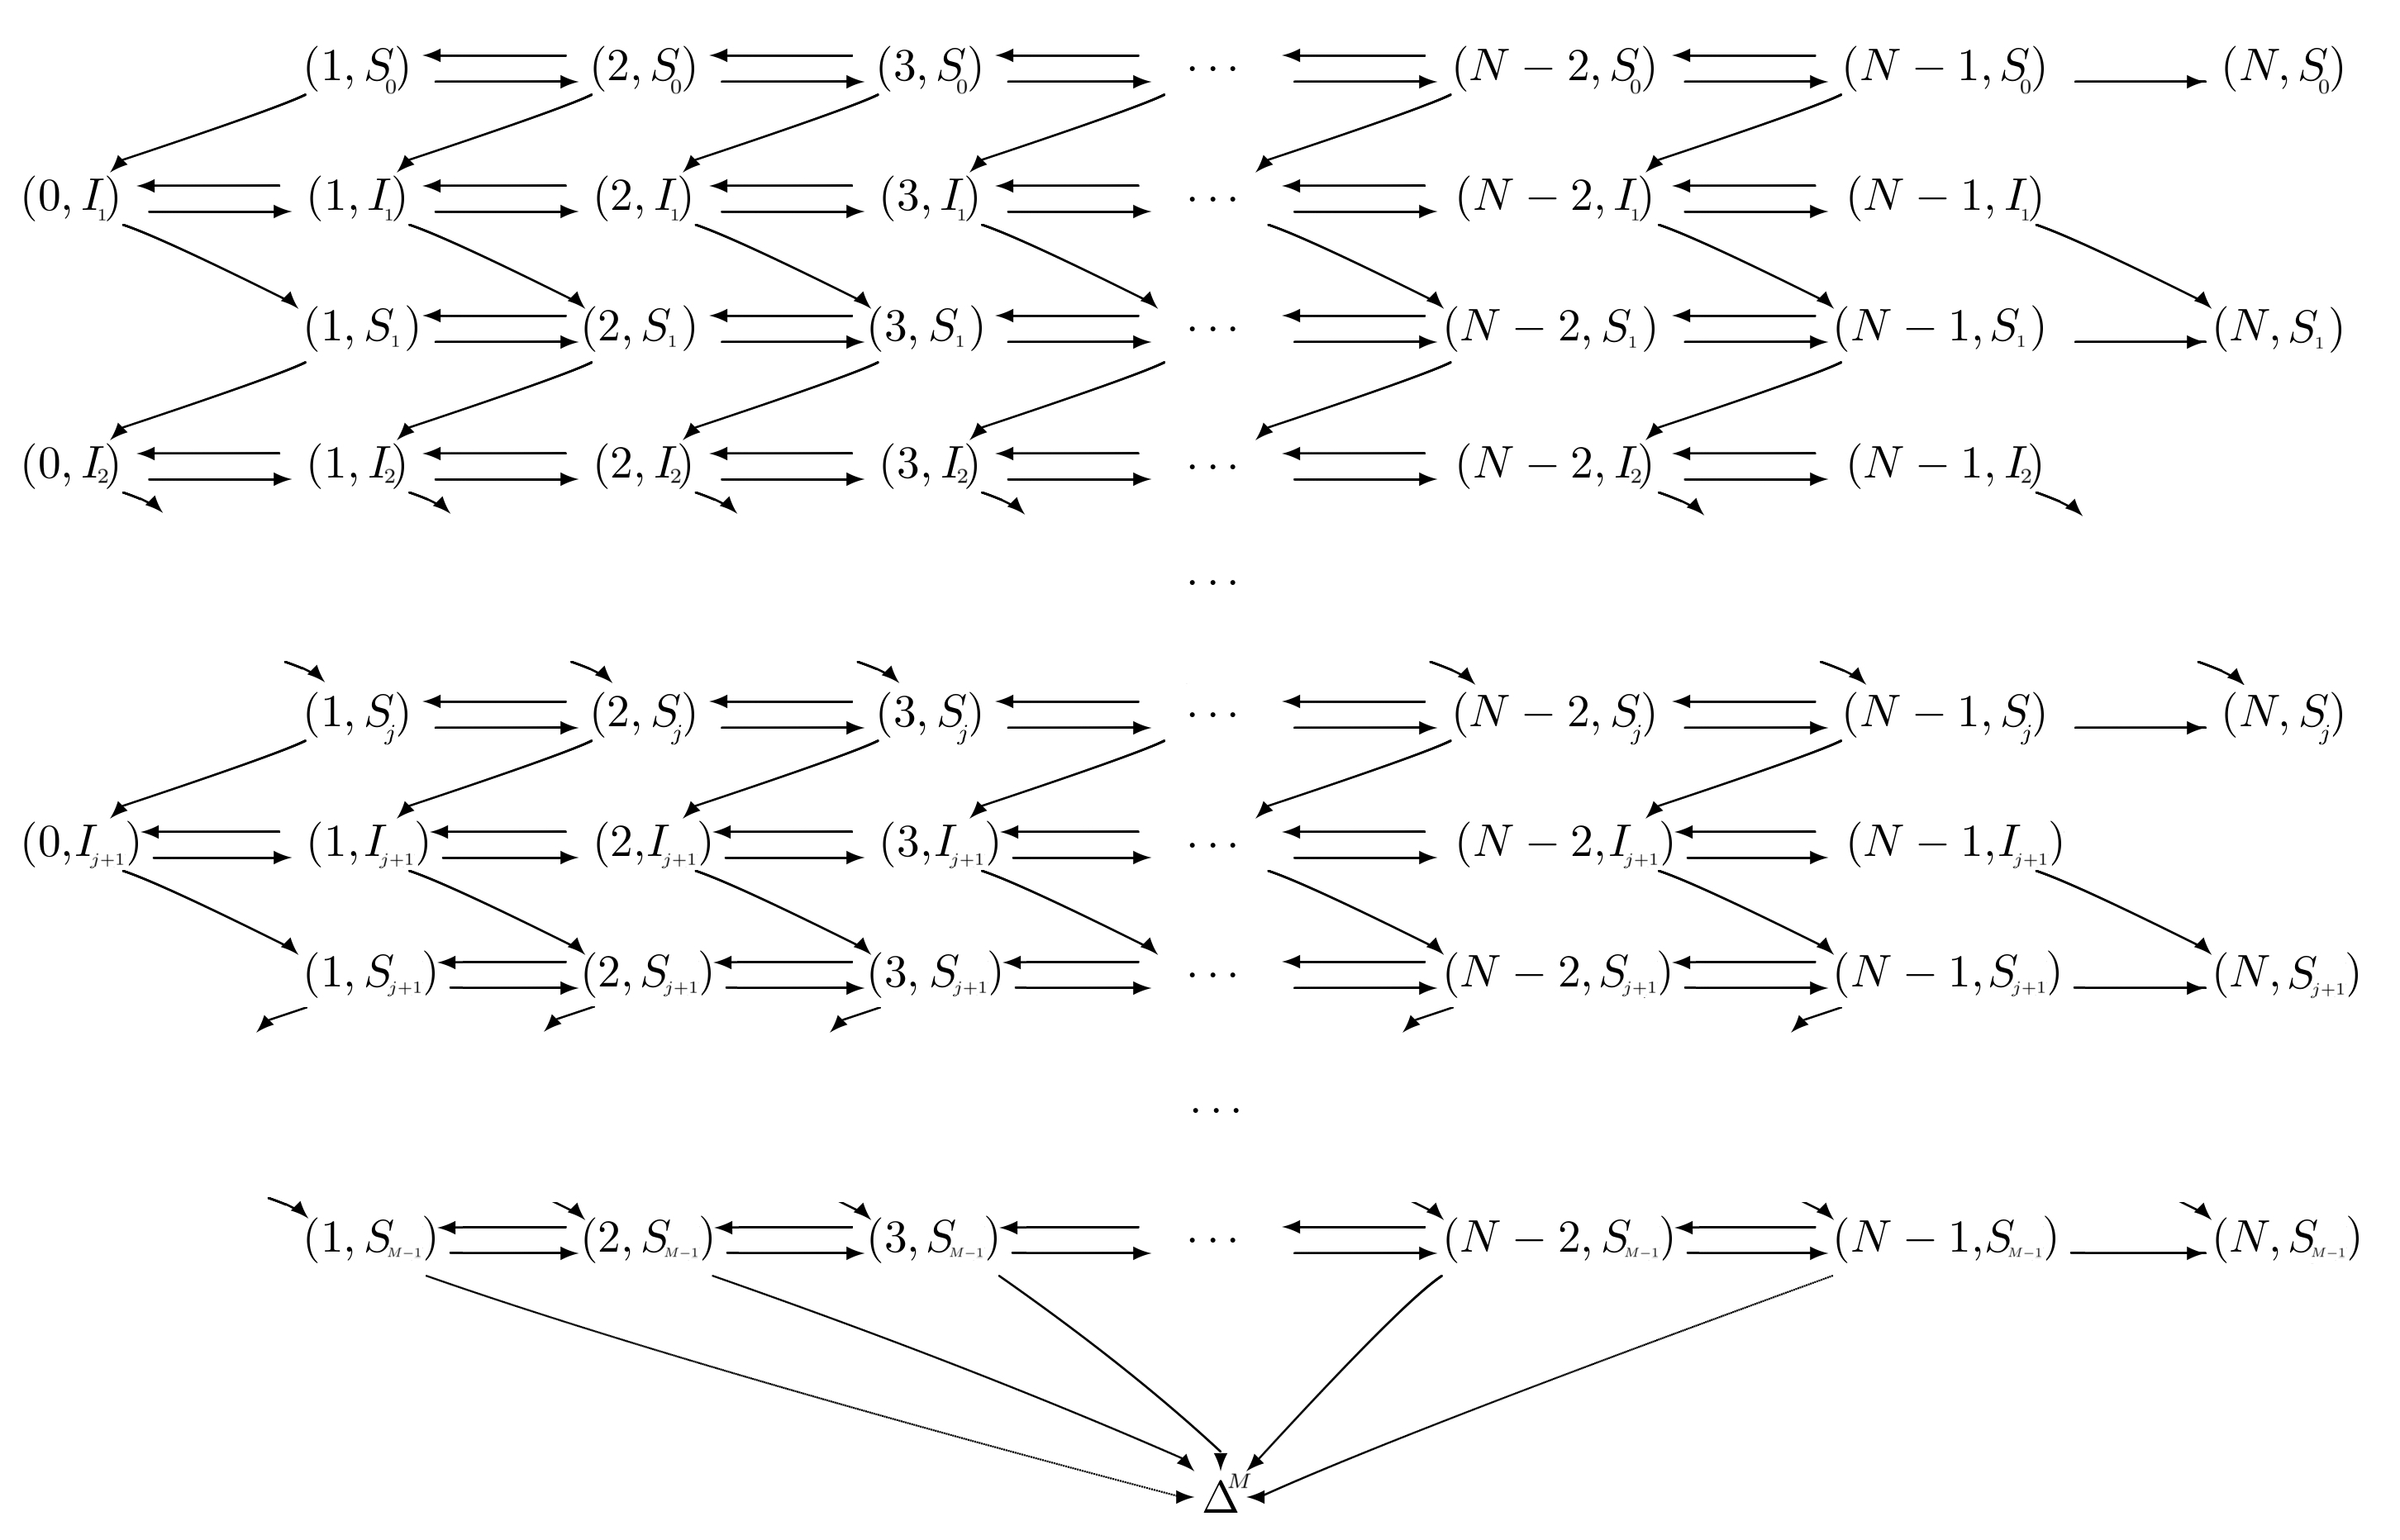
\includegraphics[width=\textwidth]{Figure3_new.jpg}
\caption{Transitions diagram of ${\cal X}^{ext,M}$.}
\label{fig:3new}
\end{figure}

\par This diagram also gives some clue on how to iteratively solve the system of equations given by $(E.S_j)-(E.I_j)$. In particular, we can start
solving Equations $(E.S_{M-1})$ for all values of $m$ and, once probabilities in this equations are in hand, Equations $(E.I_j)$ are solved after $(E.S_j)$, while Equations
$(E.S_{j-1})$ are solved after Equations $(E.I_j)$. In particular, if we developed Algorithms $S_j$ and $I_j$ (following the same arguments than in
previous section), probabilities of interest are computed as follows:

\begin{description}
  \item \it Run Algorithm $S_{M-1}$;
  \item \it For $j=M-2,\dots,0$:
  \item $~$\hspace{0.5cm} \it Run Algorithm $I_{j+1}$;
  \item $~$\hspace{0.5cm} \it Run Algorithm $S_{j}$;
\end{description}

\par\noindent with Algorithms $S_j$ and $I_j$ described below.

\newpage

%\vspace{0.5cm}
\par \noindent{\bf Algorithm $S_j$, $0\leq j\leq M-1$}\\

\begin{minipage}{9cm}
\begin{description}
  \item $h_{(N-1,S)} ~=~ 1$;
  \item $f_{(N-1,S)} ~=~ \frac{\beta(N-2)}{\theta_{(N-1,S)}}$;
  \item $g_{(N-1,S_j)} ~=~ \frac{\beta_{\cdot\rightarrow A}}{\theta_{(N-1,S)}}\left(1_{j=M-1}+1_{j<M-1}p^M_{(N-2,I_{j+1})}\right)$;
  \item \it For $m=N-2,\dots,1$:
  \item $~$\hspace{0.5cm} $h_{(m,S)} ~=~ 1-\frac{\gamma(N-m)}{\theta_{(m,S)}}h_{(m+1,S)}^{-1}f_{(m+1,S)}$;
  \item $~$\hspace{0.5cm} $f_{(m,S)} ~=~ \frac{\beta (m-1)(N-m)}{\theta_{(m,S)}}$;
\end{description}
\end{minipage}\begin{minipage}{9cm}
\begin{description}
  \item $~$\hspace{0.5cm} $g_{(m,S_j)} ~=~ \frac{\beta_{\cdot\rightarrow A}(N-m)}{\theta_{(m,S)}}\left(1_{j=M-1}+1_{j<M-1}p^M_{(m-1,I_{j+1})}\right)$\\
  \item $~$\hspace{1.8cm} $+\frac{\gamma(N-m)}{\theta_{(m,S)}}h_{(m+1,S)}^{-1}g_{(m+1,S_j)}$;
  \item $p^M_{(1,S_j)} ~=~ h_{(1,S)}^{-1}g_{(1,S_j)}$;
  \item \it For $m=2,\dots,N-1$:
  \item $~$\hspace{0.5cm} $p^M_{(m,S_j)} ~=~ h_{(m,S)}^{-1}\left(f_{(m,S)}p^M_{(m-1,S_j)}+g_{(m,S_j)}\right)$;
  \item $~$
\end{description}
\end{minipage}
\vspace{0.5cm}
\par \noindent{\bf Algorithm $I_j$, $1\leq j\leq M-1$}\\

\begin{minipage}{9cm}
\begin{description}
  \item $h_{(N-1,I)} ~=~ 1$;
  \item $f_{(N-1,I)} ~=~ \frac{\beta_{A\rightarrow\cdot}(N-1)}{\theta_{(N-1,I)}}$;
  \item $g_{(N-1,I_j)} ~=~ \frac{\gamma_A}{\theta_{(N-1,I)}}p^M_{(N,S_{j})}$;
  \item \it For $m=N-2,\dots,0$:
  \item $~$\hspace{0.5cm} $h_{(m,I)} ~=~ 1-\frac{\gamma(N-m-1)}{\theta_{(m,I)}}h_{(m+1,I)}^{-1}f_{(m+1,I)}$;
  \item $~$\hspace{0.5cm} $f_{(m,I)} ~=~ \frac{\beta m(N-m-1)+\beta_{A\rightarrow\cdot}m}{\theta_{(m,I)}}$;
\end{description}
\end{minipage}\begin{minipage}{9cm}
\begin{description}
  \item $~$\hspace{0.5cm} $g_{(m,I_j)} ~=~ \frac{\gamma_A}{\theta_{(m,I)}}p^M_{(m+1,S_j)}+\frac{\gamma(N-m-1)}{\theta_{(m,I)}}h_{(m+1,I)}^{-1}g_{(m+1,I_j)}$;
  \item $p^M_{(0,I_j)} ~=~ h_{(0,I)}^{-1}g_{(0,I_j)}$;
  \item \it For $m=1,\dots,N-1$:
  \item $~$\hspace{0.5cm} $p^M_{(m,I_j)} ~=~ h_{(m,I)}^{-1}\left(f_{(m,I)}p^M_{(m-1,I_j)}+g_{(m,I_j)}\right)$;
  \item $~$
  \item $~$
  \item $~$
\end{description}
\end{minipage}

\par\noindent We note here that $h_{(m,S)}$ and $f_{(m,S)}$ have been computed in Algorithm 1 for all values of $m$. Finally, it is worth to
point out that, once probabilities $p^M_{(m,a)}$ are in hand for different values of $M$, the probability of individual $A$
suffering exactly $M$ infections given the initial state $(m,a)$ is given by $p^M_{(m,a)}-p^{M+1}_{(m,a)}$.

\subsection{TI-, PI- and TPI-SIR models}

\par We proceed here as before and define the extended process ${\cal \tilde X}^{ext,M}=\{{\bf \tilde X}^{ext,M}(t)=({\tilde S}^M(t),{\tilde A}^M(t)):\ t\geq0\}$ where
${\tilde A}^M(t)$ takes values among $a\in\{S_0,\dots,S_{M-1},I_1,\dots,I_{M-1},R_1,\dots,R_{M-1}\}$. ${\cal \tilde X}^{ext,M}$ is defined over the
space of states
\begin{eqnarray*}
 {\cal \tilde S}^{ext,M} &=& \left({\cal \tilde S}^{ext,M}(S)\times\{S_0,\dots,S_{M-1}\}\right)\cup\left({\cal \tilde S}^{ext,M}(I)\times\{I_1,\dots,I_{M-1}\}\right)\cup\left({\cal \tilde S}^{ext,M}(R)\times\{R_1,\dots,R_{M-1}\}\right)\cup\{{\tilde \Delta}^M\},
\end{eqnarray*}
\par\noindent where ${\tilde \Delta}^M$ is the artificial absorbing state representing that individual $A$ suffered at least $M$ infections, and
where
\begin{eqnarray*}
 {\cal \tilde S}^{ext,M}(S) &=& \{(m,n)\in\mathbb{N}_0^2:\ m>0,\ m+n\leq N\},\\
{\cal \tilde S}^{ext,M}(I) &=& \{(m,n)\in\mathbb{N}_0^2:\ n>0,\ m+n\leq N\},\\
{\cal \tilde S}^{ext,M}(R) &=& \{(m,n)\in\mathbb{N}_0^2:\ m+n<N\}.
\end{eqnarray*}

\par\noindent Possible transitions among states in our extended process are given in Table \ref{tab:2new}, where states
with $n=0$ are considered as absorbing states, and where $i_{(m,n)}$, ${\bar i}_{(m,n)}$, $e_{(m,n)}$, ${\bar e}_{(m,n)}$, $r_{(m,n)}$, ${\bar r}_{(m,n)}$,
$d_{(m,n)}$, ${\bar d}_{(m,n)}$, $w_{(m,n)}$ and ${\bar w}_{(m,n)}$ are defined in previous section.

\begin{table}[h]
\centering
\begin{tabular}{|l|l|l|l|}
\hline
Type of event & Original state ($n\geq1$, $m+n\leq N$, $m\geq0$) & Destination state & Rate\\
\hline
Recovery of an infective & $(m,n,S_j)$, $m\geq1$, $0\leq j\leq M-1$ & $(m,n-1,S_j)$ & $\gamma n$\\
 & $(m,n,I_j)$, $1\leq j\leq M-1$, $n\geq2$ & $(m,n-1,I_j)$ & $\gamma(n-1)$\\
 & $(m,n,I_j)$, $1\leq j\leq M-1$ & $(m,n-1,R_j)$ & $\gamma_A$\\
 & $(m,n,R_j)$, $m+n<N$, $1\leq j\leq M-1$ & $(m,n-1,R_j)$ & $\gamma n$\\
\hline
Infection of a susceptible & $(m,n,S_{M-1})$, $m\geq1$ & ${\tilde \Delta}^M$ & $\beta_{\cdot\rightarrow A}n$\\
 & $(m,n,S_j)$, $m\geq2$, $0\leq j\leq M-1$ & $(m-1,n+1,S_j)$ & $\beta(m-1)n$\\
 & $(m,n,S_j)$, $m\geq1$, $0\leq j\leq M-2$ & $(m-1,n+1,I_{j+1})$ & $\beta_{\cdot\rightarrow A}n$\\
 & $(m,n,I_j)$, $m\geq1$, $1\leq j\leq M-1$ & $(m-1,n+1,I_j)$ & $\beta m(n-1)+\beta_{A\rightarrow\cdot}m$\\
 & $(m,n,R_j)$, $m\geq1,\ m+n<N$, $1\leq j\leq M-1$ & $(m-1,n+1,R_j)$ & $\beta mn$\\
\hline
Infection of a recovered & $(m,n,S_j)$, $m\geq1,\ m+n<N$, $1\leq j\leq M-1$ & $(m,n+1,S_j)$ & $\sigma\beta n(N-m-n)$\\
 & $(m,n,I_j)$, $m+n<N$, $1\leq j\leq M-1$ & $(m,n+1,I_j)$ & $\sigma\beta(n-1)(N-m-n)+\sigma\beta_{A\rightarrow\cdot}(N-m-n)$\\
 & $(m,n,R_j)$, $m+n<N-1$, $1\leq j\leq M-1$ & $(m,n+1,R_j)$ & $\sigma\beta n(N-m-n-1)$\\
 & $(m,n,R_j)$, $m+n<N$, $1\leq j\leq M-2$ & $(m,n+1,I_{j+1})$ & $\sigma_A\beta_{\cdot\rightarrow A} n$\\
 & $(m,n,R_{M-1})$, $m+n<N$ & ${\tilde \Delta}^{M}$ & $\sigma_A\beta_{\cdot\rightarrow A} n$\\
\hline
Immunity loss of an infective & $(m,n,S_j)$, $m\geq1$, $0\leq j\leq M-1$ & $(m+1,n-1,S_j)$ & $\alpha_I n$\\
 & $(m,n,I_j)$, $n\geq2$, $1\leq j\leq M-1$ & $(m+1,n-1,I_j)$ & $\alpha_I(n-1)$\\
 & $(m,n,I_j)$, $1\leq j\leq M-1$ & $(m+1,n-1,S_j)$ & $\alpha_I(A)$\\
 & $(m,n,R_j)$, $m+n<N$, $1\leq j\leq M-1$ & $(m+1,n-1,R_j)$ & $\alpha_I n$\\
\hline
Immunity loss of a recovered & $(m,n,S_j)$, $m\geq1,\ m+n<N$, $0\leq j\leq M-1$ & $(m+1,n,S_j)$ & $\alpha_R (N-m-n)$\\
 & $(m,n,I_j)$, $m+n<N$, $1\leq j\leq M-1$ & $(m+1,n,I_j)$ & $\alpha_R (N-m-n)$\\
 & $(m,n,R_j)$, $m+n<N-1$, $1\leq j\leq M-1$ & $(m+1,n,R_j)$ & $\alpha_R (N-m-n-1)$\\
 & $(m,n,R_j)$, $m+n<N$, $1\leq j\leq M-1$ & $(m+1,n,S_j)$ & $\alpha_R(A)$\\
\hline
\end{tabular}
\caption{Transitions among states in ${\cal \tilde S}^{ext,M}$.}
\label{tab:2new}
\end{table}

\par If we define
\begin{eqnarray*}
 p^M_{(m,n,a)} &=& \hbox{\it ``probability of individual $A$ suffering at least $M$ infections, given the current state of the process}\\
&& \hbox{\it $(m,n,a)\in{\cal \tilde S}^{ext,M}$''},
\end{eqnarray*}
\par\noindent these probabilities verify equations (for $n\geq1$, $m+n\leq N$, $m\geq0$)
\begin{eqnarray*}
 \theta_{(m,n,S)}p^M_{(m,n,S_j)} &=& \beta(m-1)np^M_{(m-1,n+1,S_j)}+\beta_{\cdot\rightarrow A}n\left(1_{j=M-1}p^M_{{\tilde \Delta}^M}+1_{j<M-1}p^M_{(m-1,n+1,I_{j+1})}\right)+\gamma np^M_{(m,n-1,S_j)}+\alpha_I n\\
&& \times p^M_{(m+1,n-1,S_j)}+\alpha_R(N-m-n)p^M_{(m+1,n,S_j)}+\sigma\beta n(N-m-n)p^M_{(m,n+1,S_j)},\quad m\geq1,\ 0\leq j\leq M-1,\ ({\tilde E}.S_j)\\
 \theta_{(m,n,I)}p^M_{(m,n,I_j)} &=& \left(\beta m(n-1)+\beta_{A\rightarrow\cdot}m\right)p^M_{(m-1,n+1,I_j)}+\gamma(n-1)p^M_{(m,n-1,I_j)}+\gamma_Ap^M_{(m,n-1,R_j)}+\alpha_I(n-1)p^M_{(m+1,n-1,I_j)}\\
&& +\alpha_I(A)p^M_{(m+1,n-1,S_j)}+\left(\sigma\beta(n-1)(N-m-n)+\sigma\beta_{A\rightarrow\cdot}(N-m-n)\right)p^M_{(m,n+1,I_j)}\\
&& +\alpha_R(N-m-n)p^M_{(m+1,n,I_j)},\quad 1\leq j\leq M-1,\quad\quad\quad\quad\quad\quad\quad\quad\quad\quad\quad\quad\quad\quad\quad\quad\quad\quad\quad\quad\quad\quad\quad\quad\quad ({\tilde E}.I_j)\\
 \theta_{(m,n,R)}p^M_{(m,n,R_j)} &=& \beta mnp^M_{(m-1,n+1,R_j)}+\gamma np^M_{(m,n-1,R_j)}+\alpha_I np^M_{(m+1,n-1,R_j)}+\alpha_R(N-m-n-1)p^M_{(m+1,n,R_j)}\\
&&+\alpha_R(A)p^M_{(m+1,n,S_j)}+\sigma\beta n(N-m-n-1)p^M_{(m,n+1,R_j)}+\sigma_A\beta_{\cdot\rightarrow A}n\\
&&\times\left(1_{j=M-1}p^M_{{\tilde \Delta}^M}+1_{j<M-1}p^M_{(m,n+1,I_{j+1})}\right),\quad m+n<N,\ 1\leq j \leq M-1,\quad\quad\quad\quad\quad\quad\quad\quad\quad\quad\quad\quad\quad\ ({\tilde E}.R_j)
\end{eqnarray*}
\par\noindent with $\theta_{(m,n,S)}$, $\theta_{(m,n,I)}$ and $\theta_{(m,n,R)}$ defined before, and boundary conditions $p^M_{{\tilde \Delta}^M}=1$, $p_{(m,0,S_j)}=p_{(m,0,R_j)}=0$ for any $m$ and $j$. These equations can be solved one after the other as follows:\\

{\centering
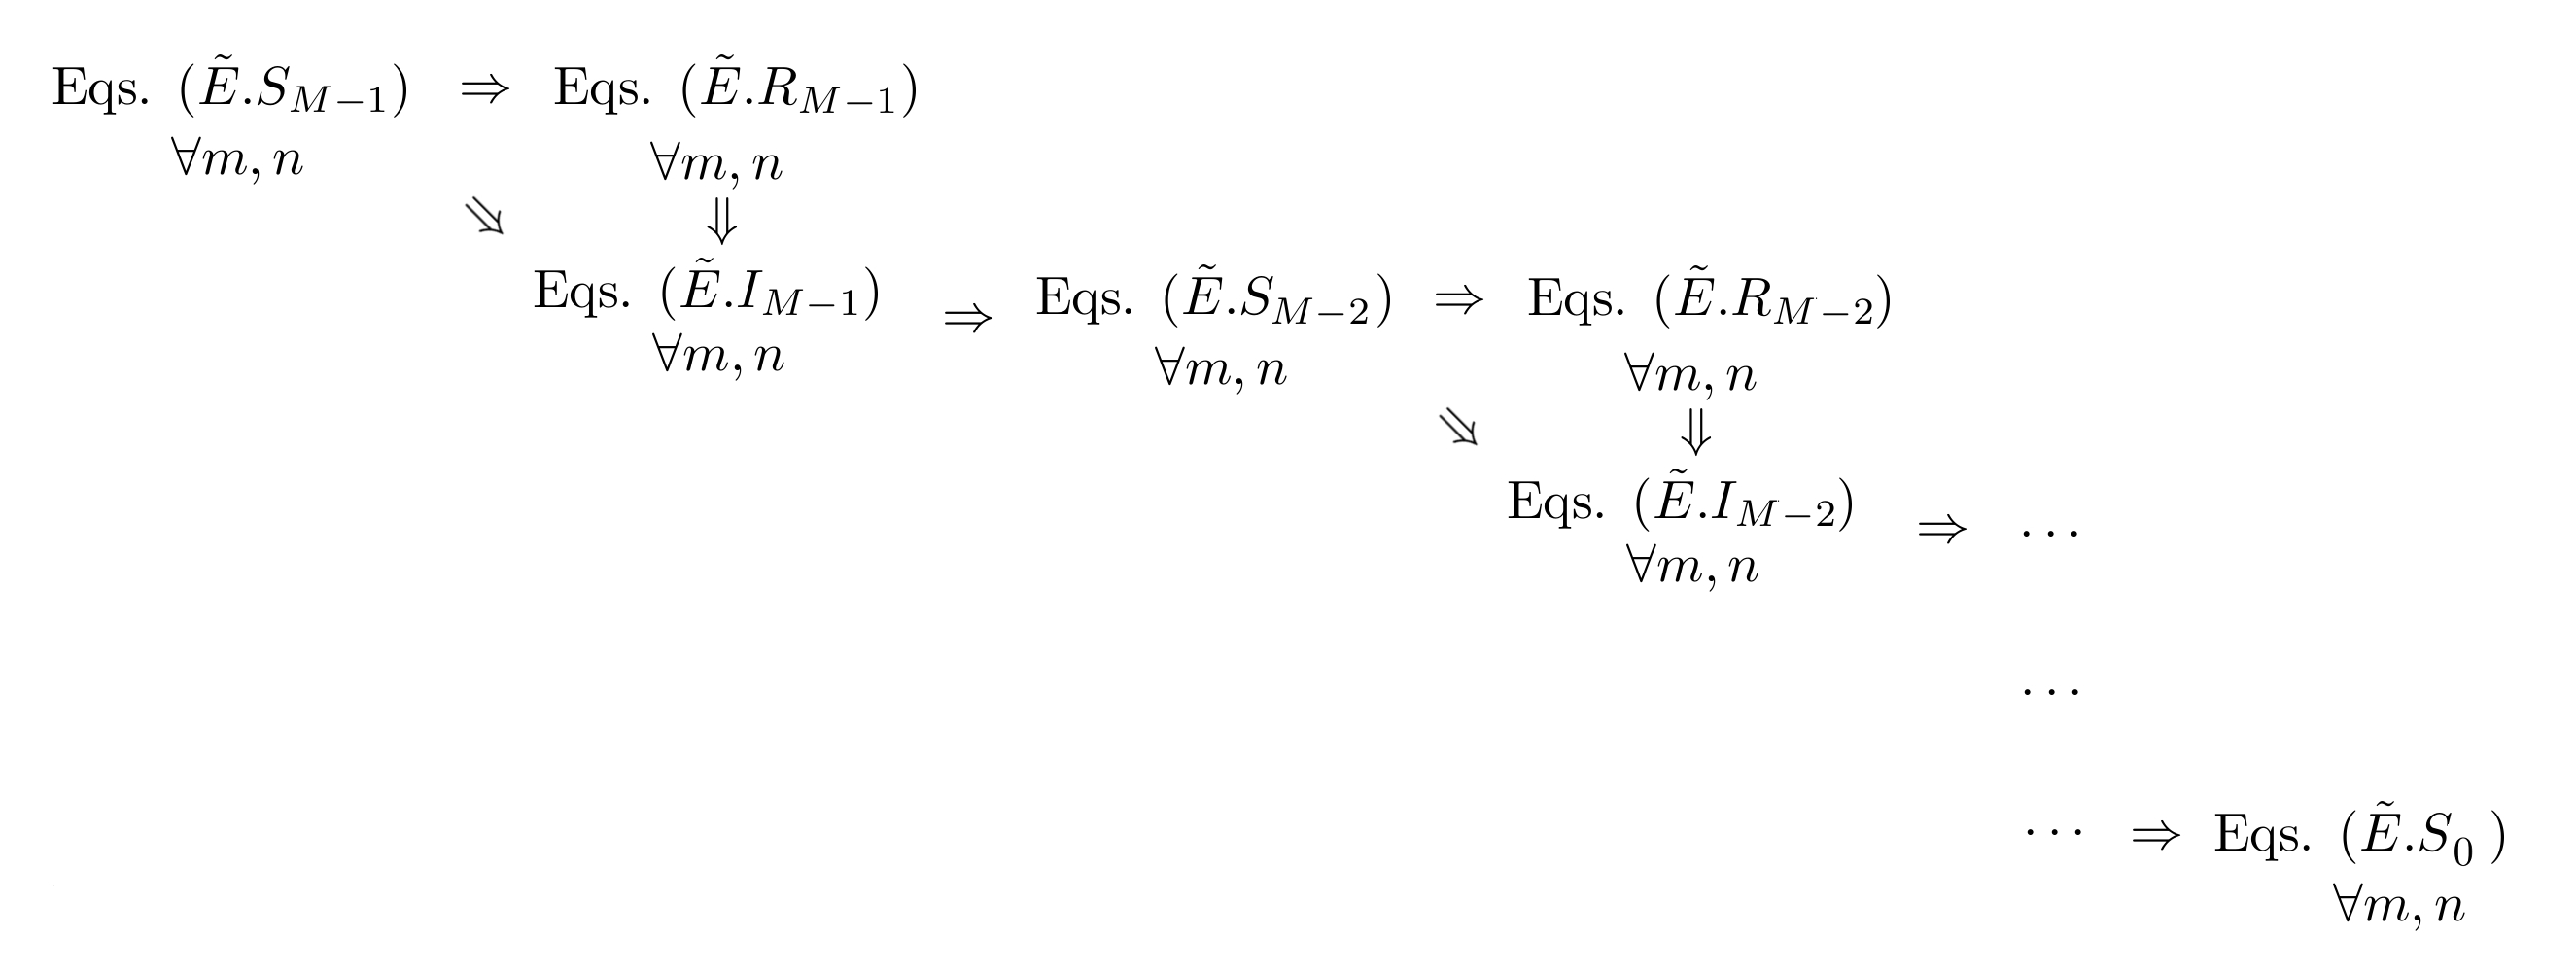
\includegraphics[width=0.8\textwidth]{FigureSolutionNew.jpg}}

\par This iterative procedure can be carried out by means of implementing a series of algorithms. In particular:

\begin{description}
  \item \it Run Algorithm ${\tilde S}_{M-1}$;
  \item \it For $j=M-2,\dots,0$:
  \item $~$\hspace{0.5cm} \it Run Algorithm ${\tilde R}_{j+1}$;
  \item $~$\hspace{0.5cm} \it Run Algorithm ${\tilde I}_{j+1}$;
  \item $~$\hspace{0.5cm} \it Run Algorithm ${\tilde S}_{j}$;
\end{description}

\par\noindent with these algorithms defined below. Algorithm ${\tilde I}_j$ follows the same steps than Algorithm ${\tilde R_j}$ but replacing matrices
and vectors ${\bf A}^M_{k,k'}(R)$ and ${\bf b}^M_k(R)$ by ${\bf A}^M_{k,k'}(I)$ and ${\bf b}^M_k(I)$, and is thus omitted.

\vspace{0.5cm}
\par \noindent{\bf Algorithm ${\tilde S_j}$}
\begin{description}
  \item ${\bf H}^M_2(S) ~=~ {\bf I}_{J(S;2)}-{\bf A}^M_{2,2}(S)$;
  \item ${\bf P}^M_2(S_j) ~=~ {\bf b}^M_2(S_j)$;
  \item \it For $k=3,\dots,N$:
  \item $~$\hspace{0.5cm} ${\bf H}^M_k(S) ~=~ {\bf I}_{J(S;k)}-{\bf A}^M_{k,k}(S)-{\bf A}^M_{k,k-1}(S){\bf H}^M_{k-1}(S)^{-1}{\bf A}^M_{k-1,k}(S)$;
  \item $~$\hspace{0.5cm} ${\bf P}^M_k(S_j) ~=~ {\bf A}^M_{k,k-1}(S){\bf H}^M_{k-1}(S)^{-1}{\bf P}^M_{k-1}(S_j)+{\bf b}^M_k(S_j)$;
  \item ${\bf p}^M_N(S_j) ~=~ {\bf H}^M_N(S)^{-1}{\bf P}^M_N(S_j)$;
  \item \it For $k=N-1,\dots,2$:
  \item $~$\hspace{0.5cm} ${\bf p}^M_k(S_j) ~=~ {\bf H}^M_k(S)^{-1}\left({\bf A}^M_{k,k+1}(S){\bf p}^M_{k+1}(S_j)+{\bf P}^M_k(S_j)\right)$;
\end{description}
\vspace{0.5cm}

\vspace{0.5cm}
\par \noindent{\bf Algorithm ${\tilde R_j}$}
\begin{description}
  \item ${\bf H}^M_1(R) ~=~ {\bf I}_{J(R;1)}-{\bf A}^M_{1,1}(R)$;
  \item ${\bf P}^M_1(R_j) ~=~ {\bf b}^M_1(R_j)$;
  \item \it For $k=2,\dots,N-1$:
  \item $~$\hspace{0.5cm} ${\bf H}^M_k(R) ~=~ {\bf I}_{J(R;k)}-{\bf A}^M_{k,k}(R)-{\bf A}^M_{k,k-1}(R){\bf H}^M_{k-1}(R)^{-1}{\bf A}^M_{k-1,k}(R)$;
  \item $~$\hspace{0.5cm} ${\bf P}^M_k(R_j) ~=~ {\bf A}^M_{k,k-1}(R){\bf H}^M_{k-1}(R)^{-1}{\bf P}^M_{k-1}(R_j)+{\bf b}^M_k(R_j)$;
  \item ${\bf p}^M_{N-1}(R_j) ~=~ {\bf H}^M_{N-1}(R)^{-1}{\bf P}^M_{N-1}(R_j)$;
  \item \it For $k=N-2,\dots,1$:
  \item $~$\hspace{0.5cm} ${\bf p}^M_k(R_j) ~=~ {\bf H}^M_k(R)^{-1}\left({\bf A}^M_{k,k+1}(R){\bf p}^M_{k+1}(R_j)+{\bf P}^M_k(R_j)\right)$;
\end{description}
\vspace{0.5cm}

\par We point out here that:
\begin{itemize}
 \item Matrices ${\bf A}^M_{k,k'}(S)={\bf A}_{k,k'}(S_I)$, ${\bf A}^M_{k,k'}(I)={\bf A}_{k,k'}(I)$ and ${\bf A}^M_{k,k'}(R)={\bf A}_{k,k'}(R)$ are
defined in previous section. Thus, matrices ${\bf H}^M_k(S)$, ${\bf H}^M_k(I)$ and ${\bf H}^M_k(R)$ are also the same than those ones
in previous section.
  \item Value of $j$ only affects matrices ${\bf P}^M_k(S_j)$, ${\bf P}^M_k(I_j)$ and ${\bf P}^M_k(R_j)$ (and not ${\bf H}^M_k(\cdot)$ matrices).
  \item Probability vectors ${\bf p}^M_k(S_j)$, ${\bf p}^M_k(I_j)$ and ${\bf p}^M_k(R_j)$ contain the desired probabilities, and are
structured and defined as vectors ${\bf p}_k(\cdot)$ in previous section.
  \item Vectors ${\bf b}^M_k(\cdot)$ are given as follows
\begin{eqnarray*}
 {\bf b}^M_k(S_j) & = & \left(\begin{array}{c}
               \frac{\beta_{\cdot\rightarrow A}}{\theta_{(k-1,1,S)}}\left(1_{j=M-1}+1_{j<M-1}p^M_{(k-2,2,I_{j+1})}\right)\\
\frac{\beta_{\cdot\rightarrow A}2}{\theta_{(k-2,2,S)}}\left(1_{j=M-1}+1_{j<M-1}p^M_{(k-3,3,I_{j+1})}\right)\\
\vdots\\
\frac{\beta_{\cdot\rightarrow A}(k-1)}{\theta_{(1,k-1,S)}}\left(1_{j=M-1}+1_{j<M-1}p^M_{(0,k,I_{j+1})}\right)\\
                         \end{array}\right),\quad 2\leq k\leq N,\quad 0\leq j\leq M-1,\\
{\bf b}^M_k(I_j) & = & \left(\begin{array}{c}
               0\\
\frac{\gamma_Ap^M_{(k-2,1,R_j)}+\alpha_I(A)p^M_{(k-1,1,S_j)}}{\theta_{(k-2,2,I)}}\\
\vdots\\
\frac{\gamma_Ap^M_{(0,k-1,R_j)}+\alpha_I(A)p^M_{(1,k-1,S_j)}}{\theta_{(0,k,I)}}
                         \end{array}\right),\quad 1\leq k\leq N,\quad 1\leq j\leq M-1,\\
{\bf b}^M_k(R_j) & = & \left(\begin{array}{c}
\frac{\alpha_R(A)p^M_{(k,1,S_j)}+\sigma_A\beta_{\cdot\rightarrow A}\left(1_{j=M-1}+1_{j<M-1}p^M_{(k-1,2,I_{j+1})}\right)}{\theta_{(k-1,1,R)}}\\
\frac{\alpha_R(A)p^M_{(k-1,2,S_j)}+2\sigma_A\beta_{\cdot\rightarrow A}\left(1_{j=M-1}+1_{j<M-1}p^M_{(k-2,3,I_{j+1})}\right)}{\theta_{(k-2,2,R)}}\\
\vdots\\
\frac{\alpha_R(A)p^M_{(1,k,S_j)}+k\sigma_A\beta_{\cdot\rightarrow A}\left(1_{j=M-1}+1_{j<M-1}p^M_{(0,k+1,I_{j+1})}\right)}{\theta_{(0,k,R)}}
                         \end{array}\right),\quad 1\leq k\leq N-1,\quad 1\leq j\leq M-1.
\end{eqnarray*}

\end{itemize}

\par\noindent Again, once probabilities $p^M_{(m,n,a)}$ are in hand for different values of $M$, the probability of individual $A$
suffering exactly $M$ infections is given by $p^M_{(m,n,a)}-p^{M+1}_{(m,n,a)}$.

\subsection{The number of individuals suffering at least $M$ infections}

\par We finally point out here that, under the homogeneous case and the ND-SIS model (these arguments also apply in the SIR models), if we mark an individual, $A$, and randomly choose the individual starting
the infection, it is clear that
\begin{eqnarray*}
\mathbb{P}(\hbox{\it $A$ suffering at least $M$ infections}) &=& p^M_{(m-1,S_0)}\frac{N-1}{N}+p^M_{(m-1,I_1)}\frac{1}{N}.
\end{eqnarray*}
\par\noindent Then, if we are interested in the random variable
\begin{eqnarray*}
 Y^M &=& \hbox{\it ``Number of individuals in the population suffering at least $M$ infections''},
\end{eqnarray*}
\par\noindent it is clear that
\begin{eqnarray*}
 \mathbb{P}(\hbox{\it $A$ suffering at least $M$ infections}) &=& \sum\limits_{y=0}^N\mathbb{P}(\hbox{\it $A$ suffering at least $M$ infections $|$ $Y^M=y$})\mathbb{P}(Y^M=y)
\end{eqnarray*}
\par\noindent and, since all the individuals are symmetric we get
\begin{eqnarray*}
 \mathbb{P}(\hbox{\it $A$ suffering at least $M$ infections}) &=& \sum\limits_{y=0}^N\frac{y}{N}\mathbb{P}(Y^M=y) \ = \ \frac{E[Y^M]}{N}
\end{eqnarray*}
\par\noindent Thus, once probabilities $p^M_{(m,a)}$ are in hand, we can easily obtain $E[Y^M]$ as
\begin{eqnarray*}
E[Y^M] &=& (N-1)p^M_{(m-1,S_0)}+p^M_{(m-1,I_1)},
\end{eqnarray*}
\par\noindent while the probability distribution of $Y^M$ could also be exactly computed, although it is out of the scope of this manuscript.

\section{Preliminary Numerical Results}

\par Here we present some preliminary numerical results, in order to illustrate the analysis developed in previous sections.

\begin{figure}
 \centering
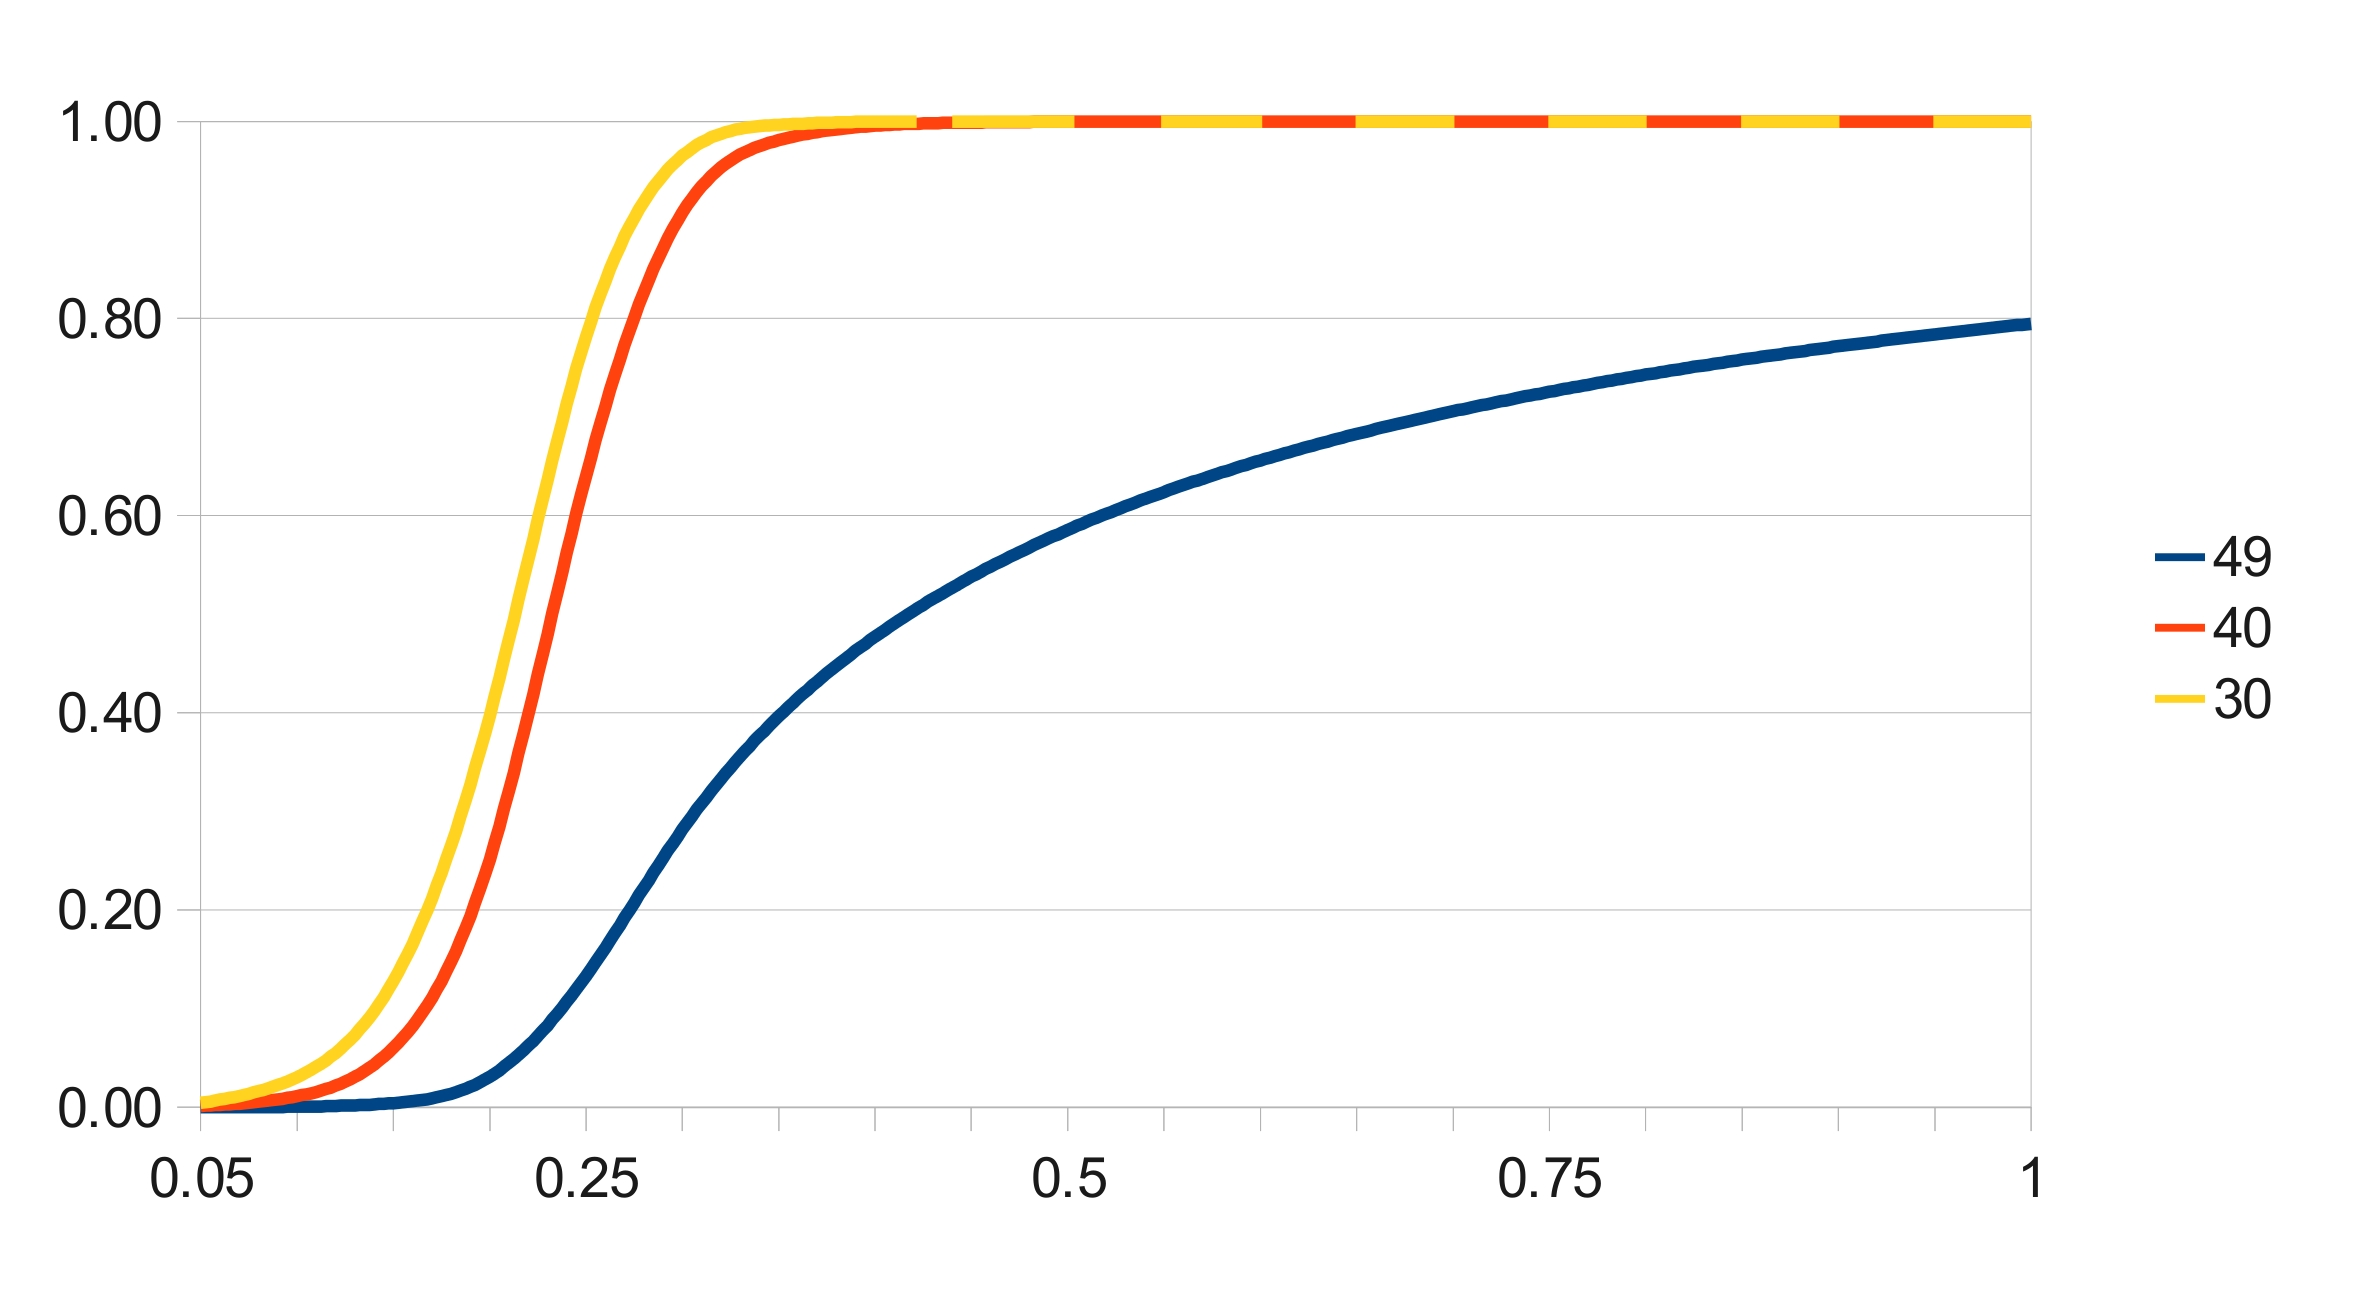
\includegraphics[width=0.5\textwidth]{Figure5.jpg}
\label{fig:5}
\caption{Individual re-infection probability of a marked individual in the ND-SIS model, for initial states $(m=49,a=S)$, $(m=40,a=S)$ and $(m=30,a=S)$,
versus $\beta$. $N=50$, $\gamma=10.0$ and completely homogeneous conditions assumed.}
\end{figure}

\begin{table}[h]
\centering
\begin{tabular}{|c|c|c|c|c|}
\hline
 &  &  & $m$ & \\
\hline
Partial Derivative & $\beta$ & $49$ & $40$ & $30$ \\
\hline
 & $0.1$ & $0.022165$ & $0.407553$ & $0.980190$ \\
\cline{2-5}
 & $0.2$ & $1.113791$ & $6.231223$ & $7.480233$ \\
\cline{2-5}
$\frac{\partial  p_{(m,S)}}{\partial \beta}$ & $0.3$ & $2.730335$ & $2.868503$ & $1.501273$ \\
\cline{2-5}
& $0.4$ & $1.382281$ & $0.121160$ & $0.014431$ \\
\cline{2-5}
& $0.5$ & $0.851877$ & $0.008741$ & $0.000126$ \\
\hline
 & $0.1$ & $-0.000222$ & $-0.004076$ & $-0.009802$ \\
\cline{2-5}
 & $0.2$ & $-0.022276$ & $-0.124624$ & $-0.149605$ \\
\cline{2-5}
$\frac{\partial  p_{(m,S)}}{\partial \gamma}$ & $0.3$ & $-0.081910$ & $-0.086055$ & $-0.045038$ \\
\cline{2-5}
& $0.4$ & $-0.055291$ & $-0.004846$ & $-0.000577$ \\
\cline{2-5}
& $0.5$ & $-0.042594$ & $-0.000437$ & $-0.000006$ \\
\hline
\end{tabular}
\caption{Partial derivatives $\frac{\partial p_{(m,S)}}{\partial \beta}$ and $\frac{\partial p_{(N-1,S)}}{\partial \gamma}$ for $\beta\in\{0.1,0.2,0.3,0.4,0.5\}$, $\gamma=10.0$
and $m\in\{49,40,30\}$. Completely homogeneous population of $N=50$ individuals.}
\label{tab:3}
\end{table}

\begin{table}[h]
\centering
\begin{tabular}{|c|c|c|c|c|}
\hline
 &  &  & $m$ & \\
\hline
Elasticity & $\beta$ & $49$ & $40$ & $30$ \\
\hline
 & $0.1$ & $4.546984$ & $3.640737$ & $3.201317$ \\
\cline{2-5}
 & $0.2$ & $7.185391$ & $4.952715$ & $3.766895$ \\
\cline{2-5}
$\frac{\frac{\partial  p_{(m,S)}}{\partial \beta}}{\frac{p_{(m,S)}}{\beta}}$ & $0.3$ & $2.907580$ & $0.948323$ & $0.466677$ \\
\cline{2-5}
& $0.4$ & $1.158382$ & $0.048682$ & $0.005774$ \\
\cline{2-5}
& $0.5$ & $0.727392$ & $0.004372$ & $0.000063$ \\
\hline
 & $0.1$ & $-4.546984$ & $-3.640737$ & $-3.201317$ \\
\cline{2-5}
 & $0.2$ & $-7.185391$ & $-4.952715$ & $-3.766895$ \\
\cline{2-5}
$\frac{\frac{\partial  p_{(m,S)}}{\partial \gamma}}{\frac{p_{(m,S)}}{\gamma}}$ & $0.3$ & $-2.907580$ & $-0.948323$ & $-0.466677$ \\
\cline{2-5}
& $0.4$ & $-1.158382$ & $-0.048682$ & $-0.005774$ \\
\cline{2-5}
& $0.5$ & $-0.727392$ & $-0.004372$ & $-0.000063$ \\
\hline
\end{tabular}
\caption{Elasticities $\frac{\frac{\partial p_{(m,S)}}{\partial \beta}}{\frac{p_{(m,S)}}{\beta}}$ and $\frac{\frac{\partial p_{(N-1,S)}}{\partial \gamma}}{\frac{p_{(N-1,S)}}{\gamma}}$ for
$\beta\in\{0.1,0.2,0.3,0.4,0.5\}$, $\gamma=10.0$ and $m\in\{49,40,30\}$. Completely homogeneous population of $N=50$ individuals.}
\label{tab:3bis}
\end{table}

\begin{figure}
 \centering
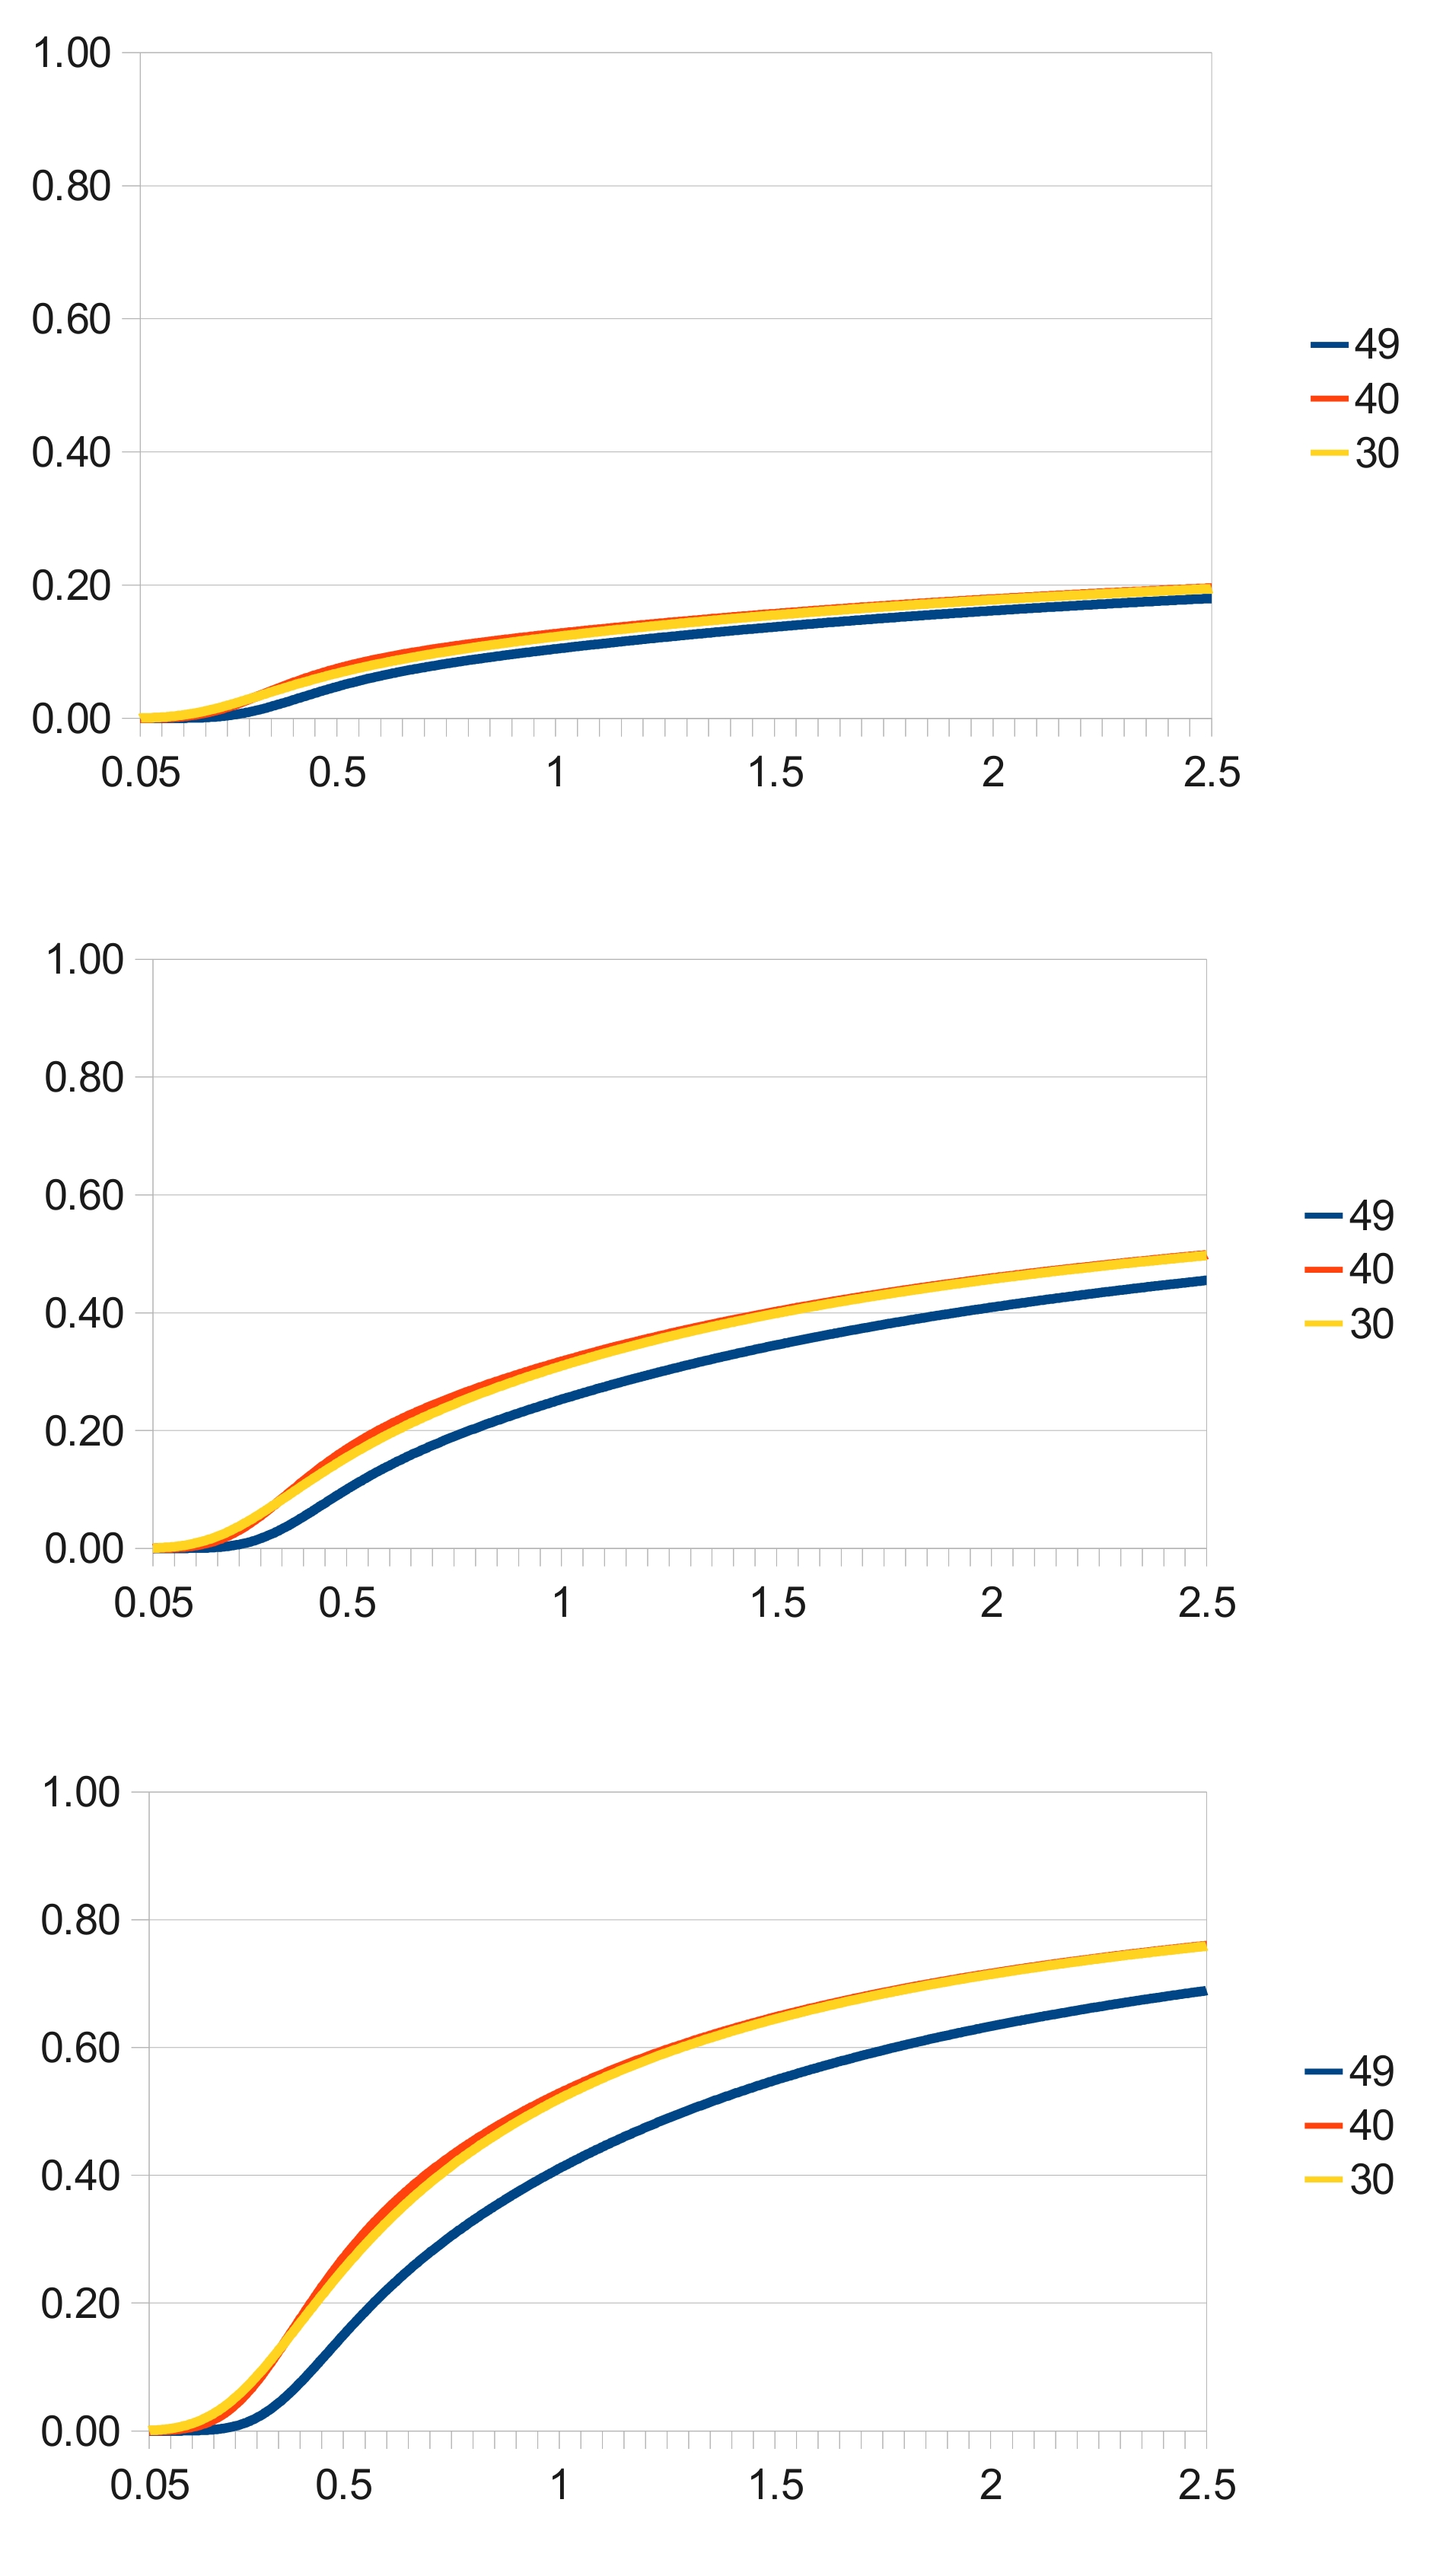
\includegraphics[width=0.5\textwidth]{Figure6.jpg}
\label{fig:6}
\caption{Individual re-infection probability of a marked individual in the TI-SIR model, for initial states $(m=49,n=1,a=S)$, $(m=40,n=10,a=S)$ and $(m=30,n=20,a=S)$,
versus $\beta$. $N=50$, $\gamma=10.0$, completely homogeneous conditions assumed and, from {\it top} to {\it bottom}, $\alpha=0.5$, $\alpha=1.0$ and
$\alpha=1.5$}
\end{figure}

\begin{table}[h]
\centering
\begin{tabular}{|c|c|c|c|c|c|}
\hline
& &  &  & $m$ & \\
\hline
$\alpha$ & Partial Derivative & $\beta$ & $49$ & $40$ & $30$ \\
\hline
 & & $0.1$ & $0.001766$ & $0.024500$ & $0.046938$ \\
\cline{3-6}
 & $\frac{\partial  p_{(m,S)}}{\partial \beta}$ & $1.0$ & $0.077692$ & $0.071199$ & $0.078480$ \\
\cline{3-6}
  & & $2.0$ & $0.042325$ & $0.037895$ & $0.038967$ \\
\cline{2-6}
 & & $0.1$ & $-0.000021$ & $-0.000305$ & $-0.000619$ \\
\cline{3-6}
$0.5$ & $\frac{\partial  p_{(m,S)}}{\partial \gamma}$ & $1.0$ & $-0.020441$ & $-0.022949$ & $-0.023252$ \\
\cline{3-6}
 &  & $2.0$ & $-0.029789$ & $-0.031443$ & $-0.031563$ \\
\cline{2-6}
 & & $0.1$ & $0.000057$ & $0.001210$ & $0.002983$ \\
\cline{3-6}
 & $\frac{\partial  p_{(m,S)}}{\partial \alpha}$ & $1.0$ & $0.253442$ & $0.316586$ & $0.308078$ \\
\cline{3-6}
 & & $2.0$ & $0.426490$ & $0.477271$ & $0.475387$ \\
\hline	
 & & $0.1$ & $0.002586$ & $0.039711$ & $0.080666$ \\
\cline{3-6}		
 & $\frac{\partial  p_{(m,S)}}{\partial \beta}$ & $1.0$ & $0.223218$ & $0.209263$ & $0.225033$ \\
\cline{3-6}		
  & & $2.0$ & $0.106888$ & $0.093271$ & $0.094984$ \\
\cline{2-6}		
 & & $0.1$ & $-0.000029$ & $-0.000469$ & $-0.001006$ \\
\cline{3-6}		
$1.0$ & $\frac{\partial  p_{(m,S)}}{\partial \gamma}$ & $1.0$ & $-0.054961$ & $-0.063630$ & $-0.064782$ \\
\cline{3-6}		
 &  & $2.0$ & $-0.072955$ & $-0.077348$ & $-0.077700$ \\
\cline{2-6}		
 & & $0.1$ & $0.000026$ & $0.000721$ & $0.001996$ \\
\cline{3-6}		
 & $\frac{\partial  p_{(m,S)}}{\partial \alpha}$ & $1.0$ & $0.326388$ & $0.427034$ & $0.422786$ \\
\cline{3-6}		
 & & $2.0$ & $0.515773$ & $0.586940$ & $0.587030$ \\
\hline		
 & & $0.1$ & $0.002889$ & $0.048258$ & $0.103129$ \\
\cline{3-6}
 & $\frac{\partial  p_{(m,S)}}{\partial \beta}$ & $1.0$ & $0.358424$ & $0.322241$ & $0.343491$ \\
\cline{3-6}
  & & $2.0$ & $0.134742$ & $0.106676$ & $0.108356$ \\
\cline{2-6}
 & & $0.1$ & $-0.000030$ & $-0.000542$ & $-0.001220$ \\
\cline{3-6}
$1.5$ & $\frac{\partial  p_{(m,S)}}{\partial \gamma}$ & $1.0$ & $-0.078884$ & $-0.091177$ & $-0.093401$ \\
\cline{3-6}
 &  & $2.0$ & $-0.080379$ & $-0.083413$ & $-0.083907$ \\
\cline{2-6}
 & & $0.1$ & $0.000010$ & $0.000394$ & $0.001259$ \\
\cline{3-6}
 & $\frac{\partial  p_{(m,S)}}{\partial \alpha}$ & $1.0$ & $0.286947$ & $0.393019$ & $0.393679$ \\
\cline{3-6}
 & & $2.0$ & $0.356206$ & $0.413852$ & $0.414904$ \\
\hline
\end{tabular}
\caption{Partial derivatives $\frac{\partial p_{(m,S)}}{\partial \beta}$ and $\frac{\partial p_{(N-1,S)}}{\partial \gamma}$ for $\beta\in\{0.1,0.2,0.3,0.4,0.5\}$, $\gamma=10.0$
and $m\in\{49,40,30\}$. Completely homogeneous population of $N=50$ individuals.}
\label{tab:4}
\end{table}

\begin{table}[h]
\centering
\begin{tabular}{|c|c|c|c|c|c|}
\hline
& &  &  & $m$ & \\
\hline
$\alpha$ & Elasticity & $\beta$ & $49$ & $40$ & $30$ \\
\hline
 & & $0.1$ & $4.321577$ & $3.180553$ & $2.617535$ \\
\cline{3-6}
 & $\frac{\frac{\partial  p_{(m,S)}}{\partial \beta}}{\frac{p_{(m,S)}}{\beta}}$ & $1.0$ & $0.744973$ & $0.559863$ & $0.639478$ \\
\cline{3-6}
  & & $2.0$ & $0.523364$ & $0.422672$ & $0.437778$ \\
\cline{2-6}
 & & $0.1$ & $-5.019562$ & $-3.965867$ & $-3.449388$ \\
\cline{3-6}
$0.5$ & $\frac{\frac{\partial  p_{(m,S)}}{\partial \gamma}}{\frac{p_{(m,S)}}{\gamma}}$ & $1.0$ & $-1.960082$ & $-1.804573$ & $-1.894623$ \\
\cline{3-6}
 &  & $2.0$ & $-1.841794$ & $-1.753501$ & $-1.772977$ \\
\cline{2-6}
 & & $0.1$ & $0.697985$ & $0.785314$ & $0.831852$ \\
\cline{3-6}
 & $\frac{\frac{\partial  p_{(m,S)}}{\partial \alpha}}{\frac{p_{(m,S)}}{\alpha}}$ & $1.0$ & $1.215109$ & $1.244710$ & $1.255145$ \\
\cline{3-6}
 & & $2.0$ & $1.318430$ & $1.330829$ & $1.335199$ \\
\hline
 & & $0.1$ & $4.240466$ & $3.189058$ & $2.664724$ \\
\cline{3-6}
 & $\frac{\frac{\partial  p_{(m,S)}}{\partial \beta}}{\frac{p_{(m,S)}}{\beta}}$ & $1.0$ & $0.882267$ & $0.658871$ & $0.726329$ \\
\cline{3-6}
  & & $2.0$ & $0.522423$ & $0.406700$ & $0.415744$ \\
\cline{2-6}
 & & $0.1$ & $-4.674571$ & $-3.768197$ & $-3.324236$ \\
\cline{3-6}
$1.0$ & $\frac{\frac{\partial  p_{(m,S)}}{\partial \gamma}}{\frac{p_{(m,S)}}{\gamma}}$ & $1.0$ & $-2.172313$ & $-2.003400$ & $-2.090933$ \\
\cline{3-6}
 &  & $2.0$ & $-1.782858$ & $-1.686350$ & $-1.700450$ \\
\cline{2-6}
 & & $0.1$ & $0.434105$ & $0.579139$ & $0.659512$ \\
\cline{3-6}
 & $\frac{\frac{\partial  p_{(m,S)}}{\partial \alpha}}{\frac{p_{(m,S)}}{\alpha}}$ & $1.0$ & $1.290046$ & $1.344530$ & $1.364604$ \\
\cline{3-6}
 & & $2.0$ & $1.260435$ & $1.279651$ & $1.284706$ \\
\hline
 & & $0.1$ & $4.151906$ & $3.178136$ & $2.691634$ \\
\cline{3-6}
 & $\frac{\frac{\partial  p_{(m,S)}}{\partial \beta}}{\frac{p_{(m,S)}}{\beta}}$ & $1.0$ & $0.872929$ & $0.609871$ & $0.660846$ \\
\cline{3-6}
  & & $2.0$ & $0.425574$ & $0.298017$ & $0.303300$ \\
\cline{2-6}
 & & $0.1$ & $-4.358226$ & $-3.567772$ & $-3.184622$ \\
\cline{3-6}
$1.5$ & $\frac{\frac{\partial  p_{(m,S)}}{\partial \gamma}}{\frac{p_{(m,S)}}{\gamma}}$ & $1.0$ & $-1.921201$ & $-1.725610$ & $-1.796948$ \\
\cline{3-6}
 &  & $2.0$ & $-1.269365$ & $-1.165141$ & $-1.174317$ \\
\cline{2-6}
 & & $0.1$ & $0.206320$ & $0.389636$ & $0.492987$ \\
\cline{3-6}
 & $\frac{\frac{\partial  p_{(m,S)}}{\partial \alpha}}{\frac{p_{(m,S)}}{\alpha}}$ & $1.0$ & $1.048272$ & $1.115739$ & $1.136102$ \\
\cline{3-6}
 & & $2.0$ & $0.843791$ & $0.867125$ & $0.871017$ \\
\hline
\end{tabular}
\caption{Elasticities $\frac{\frac{\partial p_{(m,S)}}{\partial \beta}}{\frac{p_{(m,S)}}{\beta}}$ and $\frac{\frac{\partial p_{(N-1,S)}}{\partial \gamma}}{\frac{p_{(N-1,S)}}{\gamma}}$ for $\beta\in\{0.1,0.2,0.3,0.4,0.5\}$, $\gamma=10.0$
and $m\in\{49,40,30\}$. Completely homogeneous population of $N=50$ individuals.}
\label{tab:5}
\end{table}


\begin{thebibliography}{5}

\bibitem{Caswell11}
Caswell H (2011)
Perturbation analysis of continuous-time absorbing Markov chains.
Numerical Linear Algebra with Applications 19: 901-917.

\bibitem{Gomes04}
Gomes MGM, White LJ, Medley GF (2004)
Infection, reinfection and vaccination under suboptimal immune protection: epidemiological perspectives.
Journal of Theoretical Biology 228: 539-549.

\bibitem{GomezCorral15}
G\'omez-Corral A, L\'opez-Garc\'ia M (2015)
Lifetime and reproduction of a marked individual in a two-species competition process.
Applied Mathematics and Computation 264: 223-245.

\bibitem{LopezGarcia15}
L\'opez-Garc\'ia M (2015)
Perturbation analysis in finite-state level-dependent QBD processes: a matrix-algorithmic approach.
In preparation.

\end{thebibliography}

\end{document} 